\chapter{HASIL DAN PEMBAHASAN}
Pada subbab pertama pada bab ini akan dipaparkan hasil akhir dari pengerjaan tugas akhir Interoperabilitas NFT Berbasis \emph{Blockchain} Menggunakan \emph{Smart Contract} pada WEB3.0. Pada subbab selanjutnya akan dipaparkan mengenai hasil pengujian dari hasil tugas akhir untuk memastikan bahwa sistem yang dikembangkan berjalan dengan sesuai.

\section{Hasil}
Hasil keseluruhan dari sistem yang dikembangkan adalah \emph{interface} berupa web, \emph{Non-Fungible Token} (NFT) dan juga \emph{smart contract} yang berinteroperabilitas. Berikut dipaparkan masing-masing hasil dari sistem yang dikembangkan.

\subsection{Web Interface}
Tampilan awal web \emph{interface}, menampilkan daftar koleksi NFT yang dapat di-\emph{minting}. Nantinya NFT tersebut dapat dimiliki oleh \emph{address} yang melakukan pertama kali \emph{minting} dan juga kepemilikan dari NFT tersebut dapat diberikan ke \emph{address} lain.
\begin{figure} [H] \centering
  % Nama dari file gambar yang diinputkan
  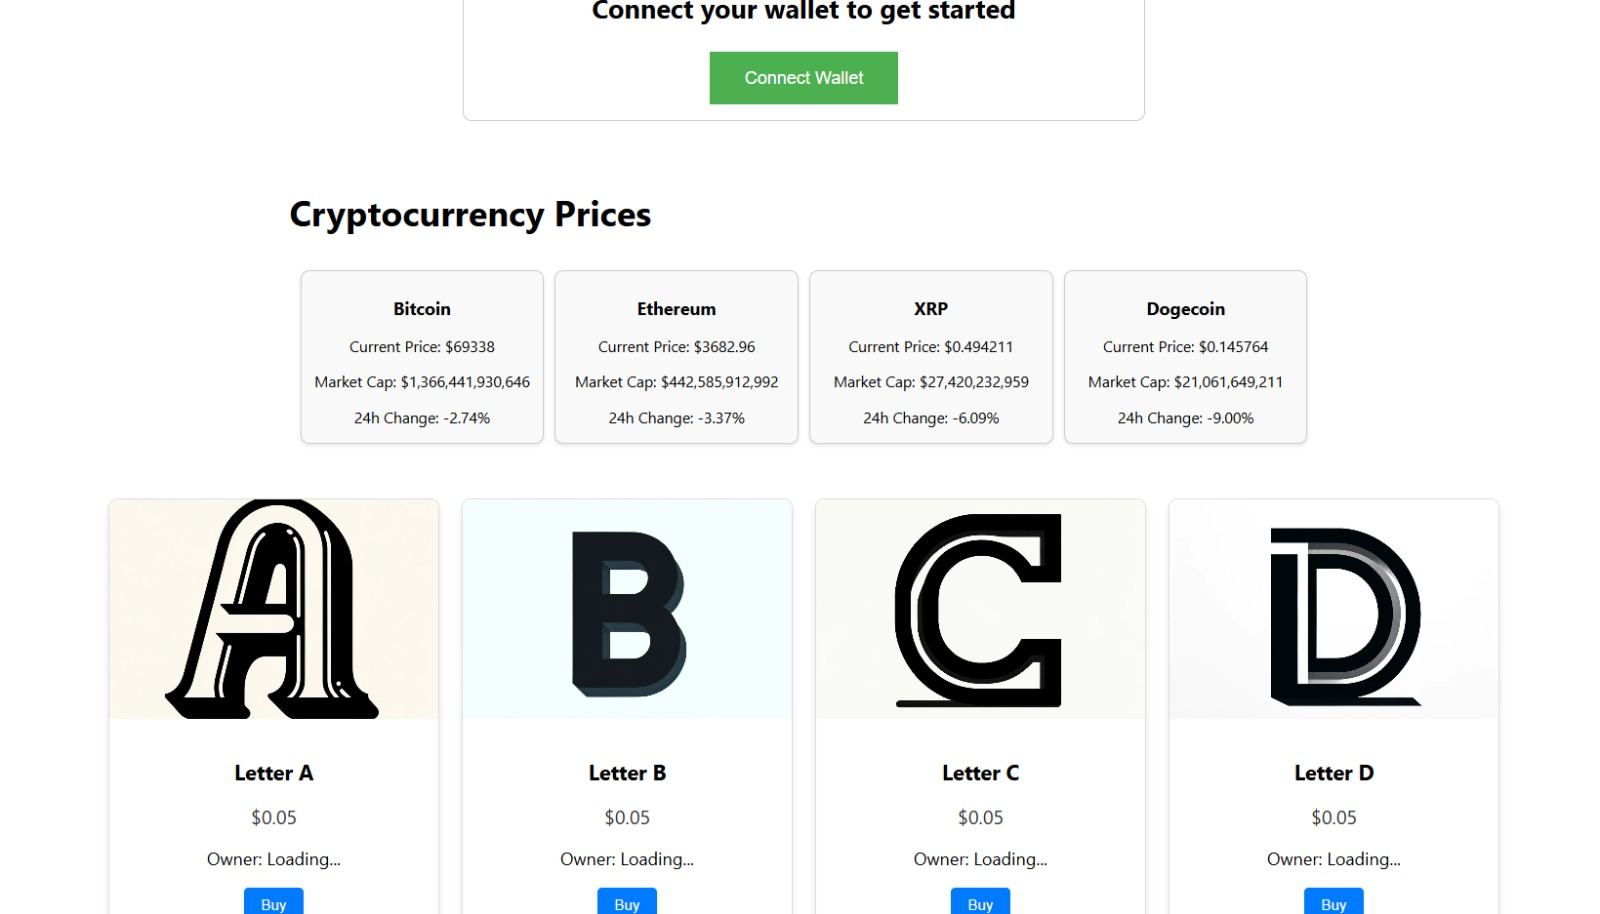
\includegraphics[scale=0.28]{gambar/web_interface.jpeg}
  % Keterangan gambar yang diinputkan
  \caption{Tampilan interface}
  % Label referensi dari gambar yang diinputkan
  \label{fig:interface}
\end{figure}

Pada dashboard awalnya pengguna harus menekan tombol \emph{Connect Wallet} yang kemudian akan terhubung dengan akun Metamask Wallet. Dari koneksi tersebut pengguna mendapatkan \emph{address} yang dapat digunakan untuk melakukan \emph{minting} token NFT.

\begin{figure} [H] \centering
  % Nama dari file gambar yang diinputkan
  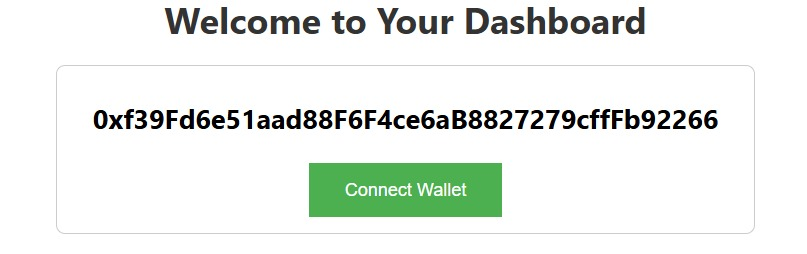
\includegraphics[scale=0.45]{gambar/dashboard_connected.jpeg}
  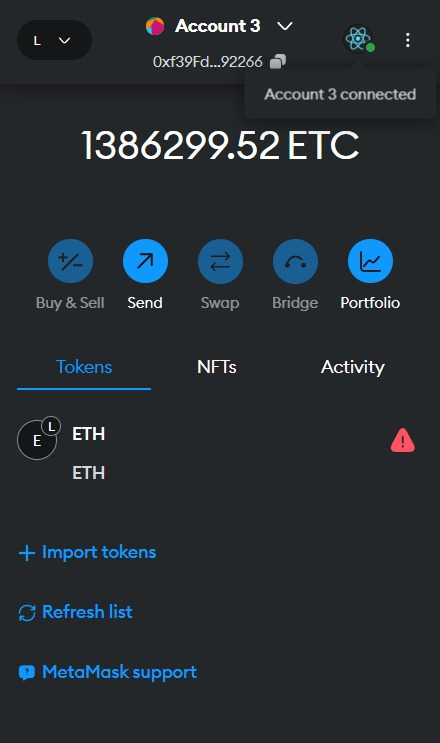
\includegraphics[scale=0.35]{gambar/metamask_connected.jpeg}
  % Keterangan gambar yang diinputkan
  \caption{Koneksi \emph{interface} dengan Metamask Wallet}
  % Label referensi dari gambar yang diinputkan
  \label{fig:koneksi_metamask}
\end{figure}

Setelah melakukan proses koneksi dengan Metamask, pengguna dapat melakukan \emph{minting} pada NFT yang tersedia pada \emph{interface} dengan menekan tombol \emph{pay}.

\begin{figure} [H] \centering
  % Nama dari file gambar yang diinputkan
  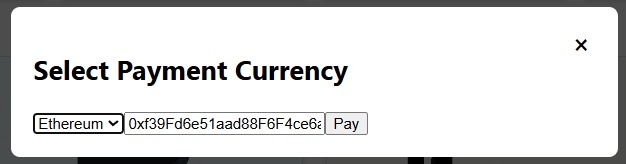
\includegraphics[scale=0.50]{gambar/payment.jpeg}
  % Keterangan gambar yang diinputkan
  \caption{\emph{Payment} dan \emph{address}}
  % Label referensi dari gambar yang diinputkan
  \label{fig:payment}
\end{figure}

Kemudian pada saat pengguna melakukan proses pembelian atau \emph{minting}, pengguna dapat memilih pembayaran dengan \emph{cryptocurrency} mana dan juga memasukkan \emph{address} untuk dapat mencetak kepemilikan NFT tersebut.

\begin{figure} [H] \centering
  % Nama dari file gambar yang diinputkan
  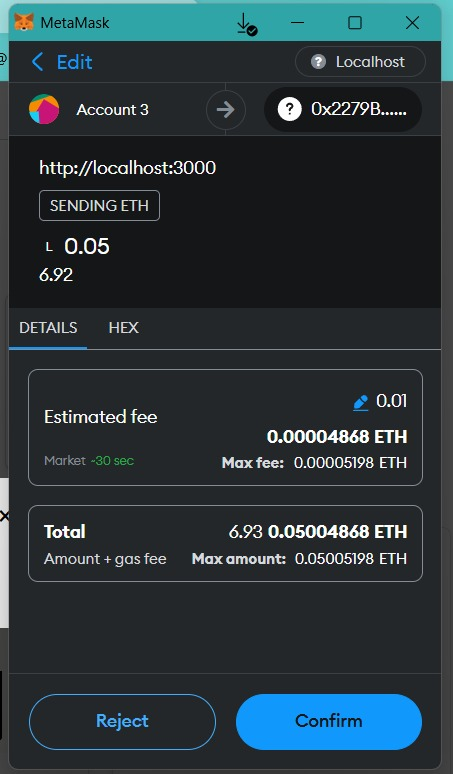
\includegraphics[scale=0.35]{gambar/transaction.jpeg}
  % Keterangan gambar yang diinputkan
  \caption{Detail \emph{payment} menggunakan Metamask Wallet}
  % Label referensi dari gambar yang diinputkan
  \label{fig:transaction}
\end{figure}

\vspace{-10pt}
Setelah melakukan proses pembayaran dan transaksi berhasil, maka pada \emph{interface} bagian \emph{owner} dari produk NFT tersebut akan diperbarui menjadi \emph{address} dari pemilik yang baru.

\begin{figure} [H] \centering
  % Nama dari file gambar yang diinputkan
  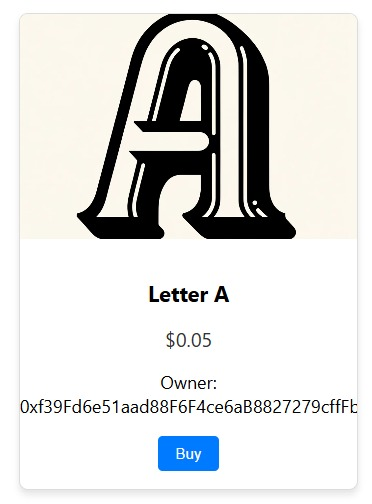
\includegraphics[scale=0.45]{gambar/new_owner.jpeg}
  % Keterangan gambar yang diinputkan
  \caption{\emph{address} pemilik baru dari NFT}
  % Label referensi dari gambar yang diinputkan
  \label{fig:owner}
\end{figure}

\subsection{\emph{Smart Contract}}
Dalam pengembangan aplikasi berbasis \emph{blockchain}, pengintegrasian \emph{smart contract} dengan antarmuka pengguna seperti React.js menjadi krusial. \emph{Smart contract} yang dibangun menggunakan Solidity dapat di-\emph{deploy} di \emph{testnet} Ethereum, seperti Sepolia Testnet, yang menyediakan lingkungan yang hampir mirip dengan mainnet Ethereum namun tanpa memerlukan biaya transaksi yang besar. 

ABI atau \emph{Application Binary Interface}, adalah cara yang memungkinkan fungsi dalam \emph{smart contract} Ethereum untuk berkomunikasi dengan aplikasi eksternal, termasuk antarmuka pengguna yang dibangun dengan kerangka kerja seperti React.js. ABI berperan sebagai lapisan translasi yang menguraikan cara memanggil fungsi dalam smart contract, jenis parameter yang diterima, jenis keluaran yang diharapkan, serta sifat state dari fungsi tersebut. ABI biasanya dihasilkan secara otomatis oleh \emph{compiler} Solidity sebagai bagian dari proses kompilasi \emph{smart contract} dan disimpan dalam format JSON. Setiap kali aplikasi \emph{frontend} mengirimkan transaksi atau \emph{query} ke \emph{blockchain}, ia menggunakan ABI untuk mengkodekan data panggilan ke dalam format yang dapat dipahami oleh \emph{Ethereum Virtual Machine} (EVM). Kemudian, saat data dikembalikan dari \emph{smart contract}, ABI digunakan untuk mendekode balasan sehingga aplikasi React.js dapat memahami dan memprosesnya.

Proses \emph{deploy} dilakukan \emph{smart contract} akan di-\emph{deploy} ke beberapa jaringan \emph{blockchain} namun dikarenakan dalam pengujian ini yang digunakan adalah sepolia \emph{testnet} maka yang digunakan hanyalah dari jaringan sepolia \emph{testnet}. Ketika melakukan proses \emph{deployment} akan dikenakan \emph{gas} atau fee yang dapat dibayar menggunakan \emph{ethereum} yang terdapat pada \emph{wallet} Metamask. Yang kemudian detail dari transaksi tersebut dapat dilihat pada Etherscan.

\begin{figure} [H] \centering
  % Nama dari file gambar yang diinputkan
  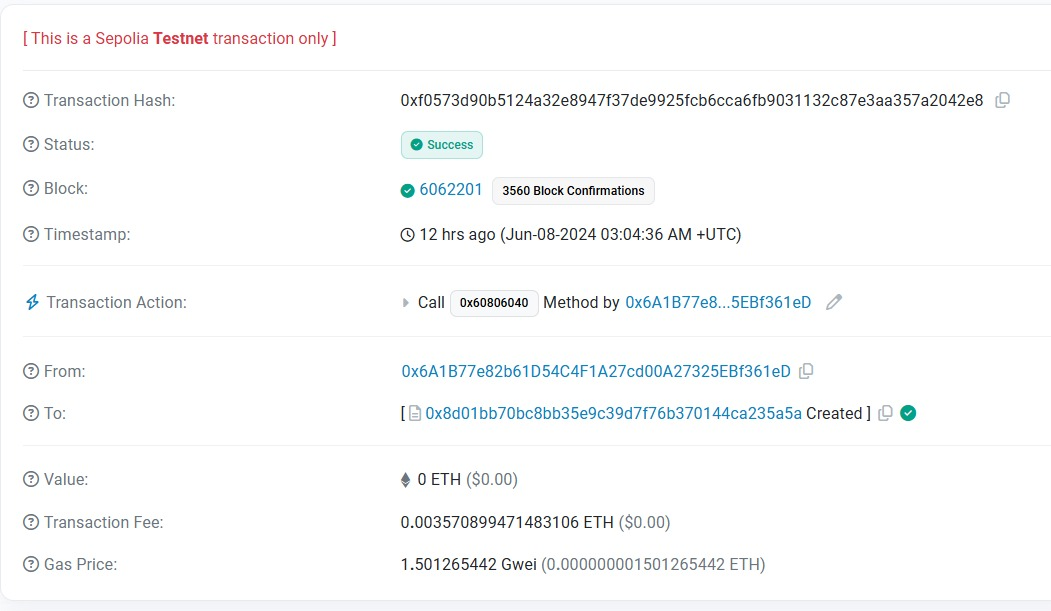
\includegraphics[scale=0.45]{gambar/etherscan.jpeg}
  % Keterangan gambar yang diinputkan
  \caption{Detail transaksi pada etherscan}
  % Label referensi dari gambar yang diinputkan
  \label{fig:transaction}
\end{figure}

\subsection{\emph{Non-Fungible Token} (NFT)}
\emph{Non-Fungible Token} (NFT) sendiri juga memiliki beberapa tahapan agar dapat dapat disimpan dalam \emph{The Interplanetary File System} (IPFS) dan kemudian dapat di-\emph{publish} pada OpenSea \emph{test net}. Pada pengerjaan tugas akhir ini, Pinata digunakan sebagai \emph{platform} untuk mengunggah foto NFT dan juga data \emph{JavaScript Object Notation} (JSON) agar bisa di-\emph{minting} sebagai \emph{Uniform Resource Identifier} (URI) pada \emph{smart contract}. Hal ini dibutuhkan agar NFT yang di-\emph{minting} memiliki gambar yang dapat dilihat pada OpenSea.

\begin{figure} [H] \centering
  % Nama dari file gambar yang diinputkan
  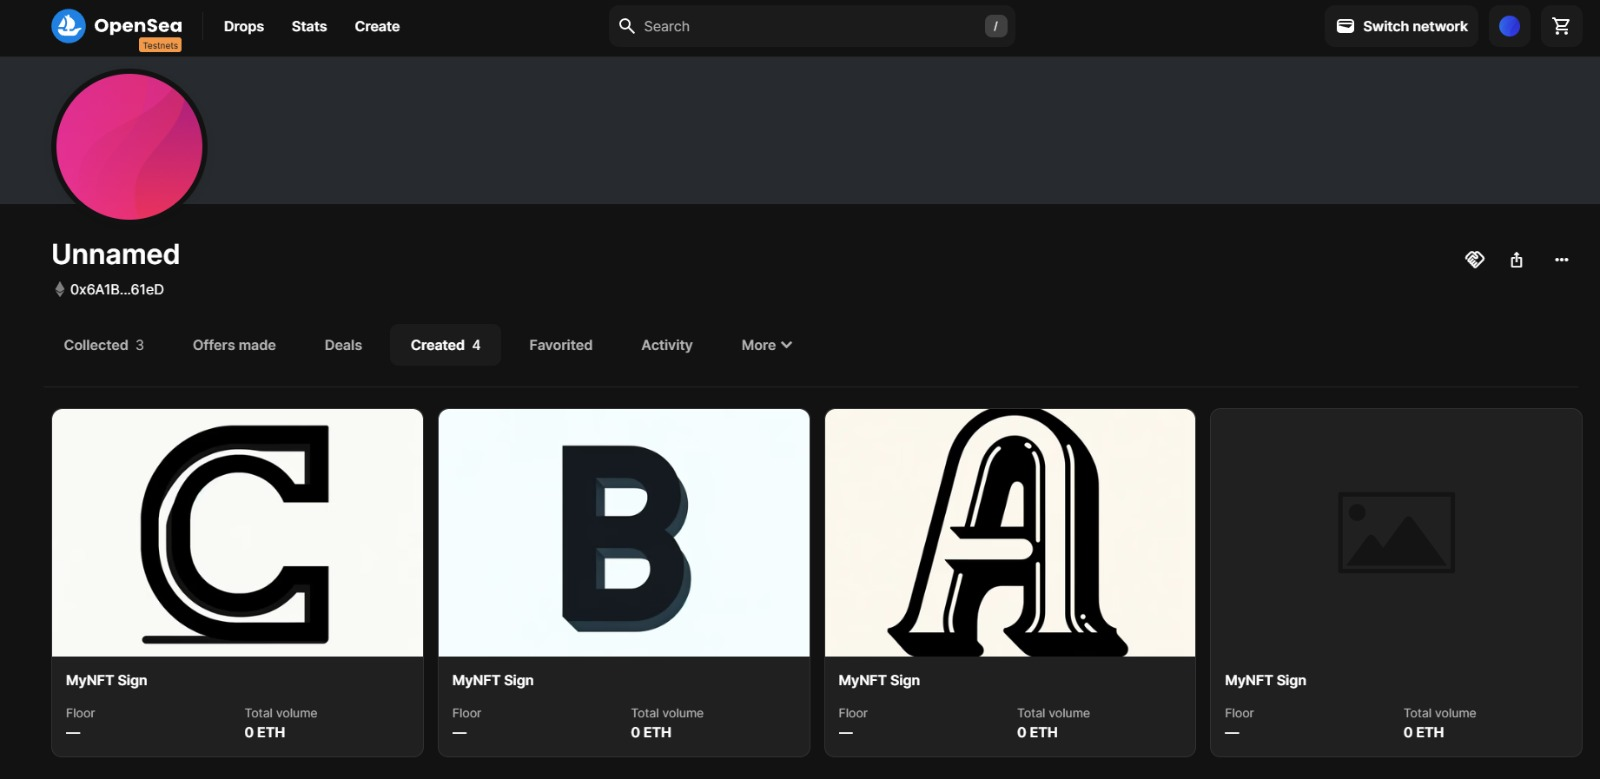
\includegraphics[scale=0.28]{gambar/opensea.jpeg}
  % Keterangan gambar yang diinputkan
  \caption{NFT terunggah pada Opensea}
  % Label referensi dari gambar yang diinputkan
  \label{fig:opensea}
\end{figure}

\section{Pengujian}
Untuk memastikan bahwa sistem interoperabilitas \emph{Smart Contract} berjalan sesuai dengan yang direncakan maka perlu dilakukan pengujian lebih lanjut. Pengujian yang dilakukan secara garis besar dibagi menjadi dua yaitu Pengujian fitur-fitur utama dari \emph{Smart Contract} yang meliputi \emph{minting}, \emph{lock}, dan \emph{bridge transfer} kepemilikan NFT dan yang kedua adalah pengujian integrasi ke \emph{interface} yang telah dibuat. Berikut merupakan paparan dari pengujian.

\subsection{Pengujian Fitur \emph{Smart Contract}}
Ekspektasi pengujian dari sistem \emph{smart contract} antara lain adalah sebagai berikut:
\begin{itemize}
    \item \emph{User} dapat melakukan minting token NFT yang kemudian kepemilikan NFT tersebut dapat dilihat pada \emph{test net} \emph{platform} OpenSea.

    \item Antar \emph{user} yang berbeda \emph{Network} dapat saling berkomunikasi dan kepemilikan \emph{token} NFT dapat berpindah dari \emph{user} A yang berada pada \emph{network} A' ke \emph{user} B yang berada pada \emph{network} B'.
\end{itemize}

Berikut merupakan data mengenai \emph{wallet} yang digunakan dalam pengujian:

\begin{center}
\begin{table}[H]
      \centering
      \caption{Informasi Akun}
      \begin{tabular}{|c|c|c|}
      \hline
      \textbf{Akun} & \textbf{Address} & \textbf{\emph{Network}}
      \\
      \hline
      A & 0x6A1B77e82b61D54C4F1A27cd00A27325EBf361eD & \emph{Sepolia Ethereum Testnet}
      \\ 
      \hline
      B & 0xD066d6576D9485Eb2c2a41BB8B52EcE17a0557d6 & \emph{BNB Chain Testnet} \\
      \hline
      \end{tabular}      
      \label{tab:hardware-specs}
\end{table}
\end{center}

Berikut merupakan langkah-langkah dari pengujian sistem \emph{smart contract} yang akan dilakukan:

\begin{itemize}
    \item \emph{User} A akan melakukan \emph{minting} pada NFT terlebih dahulu

    \begin{figure} [H] \centering
    % Nama dari file gambar yang diinputkan
    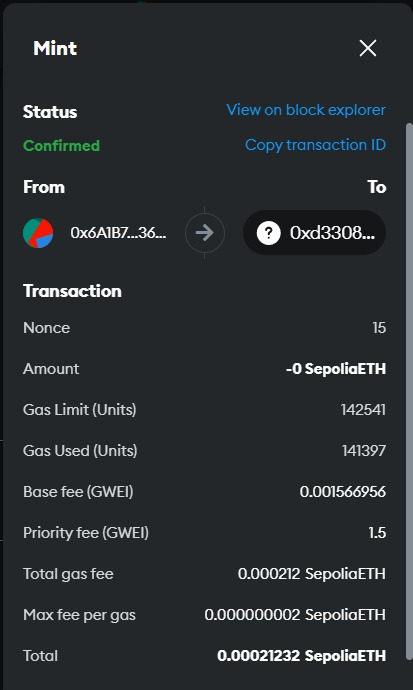
\includegraphics[scale=0.35]{gambar/riwayat_transaksi.jpeg}
    % Keterangan gambar yang diinputkan
    \caption{Riwayat transaksi minting pada Metamask Wallet}
    % Label referensi dari gambar yang diinputkan
    \label{fig:minting}
    \end{figure}

    \item dapat dilihat juga pada gambar di bawah terdapat detail pada etherscan yang menunjukkan detail seperti \emph{transaction hash}, \emph{block}, dan tipe dari token yaitu \emph{ERC-721}.

    \begin{figure} [H] \centering
    % Nama dari file gambar yang diinputkan
    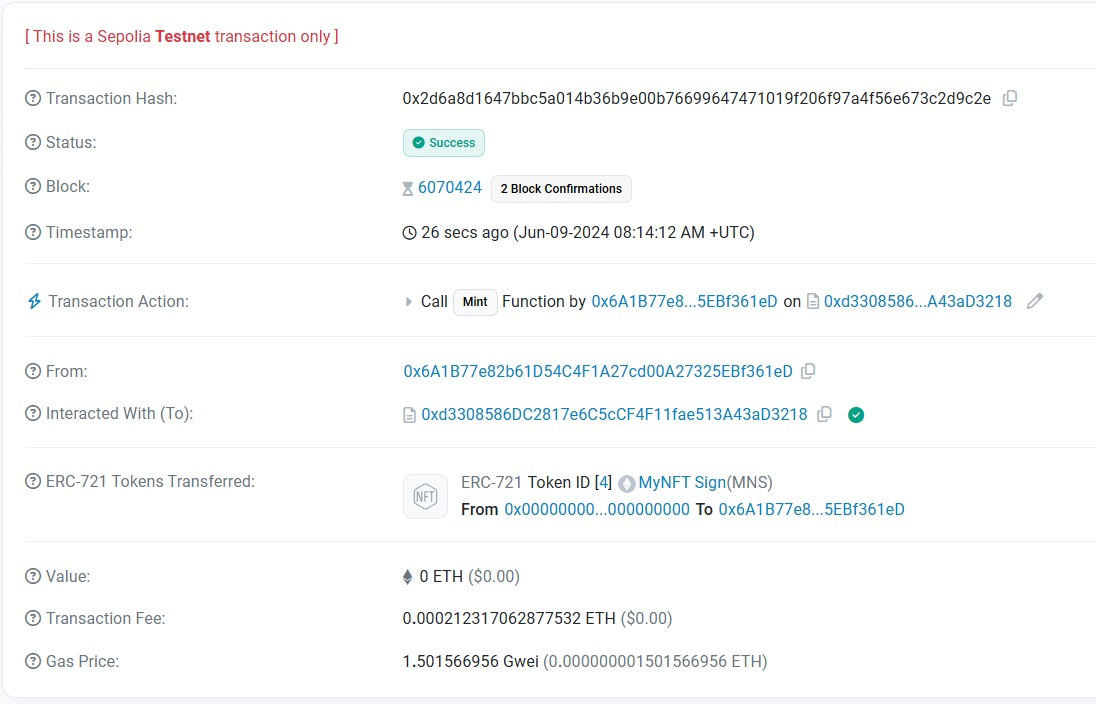
\includegraphics[scale=0.32]{gambar/detail_transaksi_etherscan.jpeg}
    % Keterangan gambar yang diinputkan
    \caption{Detail transaksi pada Etherscan}
    % Label referensi dari gambar yang diinputkan
    \label{fig:detail_transaksi_etherscan}
    \end{figure}

    \item kemudian pada etherscan juga terdapat detail dari NFT yang telah di-\emph{minting}, yang dapat dilihat seperti pada gambar berikut

    \begin{figure} [H] \centering
    % Nama dari file gambar yang diinputkan
    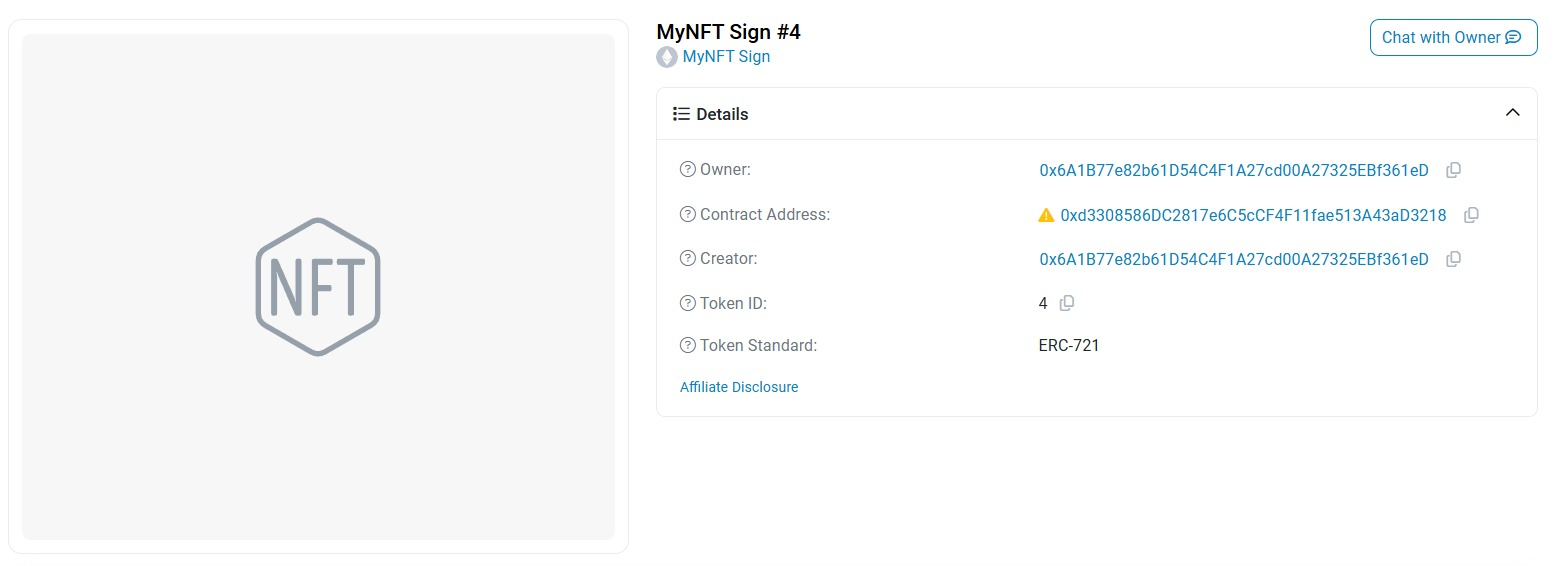
\includegraphics[scale=0.3]{gambar/detail_nft_etherscan.jpeg}
    % Keterangan gambar yang diinputkan
    \caption{Detail NFT pada Etherscan}
    % Label referensi dari gambar yang diinputkan
    \label{fig:detail_nft_etherscan}
    \end{figure}

    \item setelah proses tersebut berhasil, maka pada \emph{platform} Opensea bisa dilihat NFT yang telah di-\emph{minting}. Pada kasus pengujian ini, NFT yang ter-\emph{minting} adalah "\emph{Letter D}".

    \begin{figure} [H] \centering
    % Nama dari file gambar yang diinputkan
    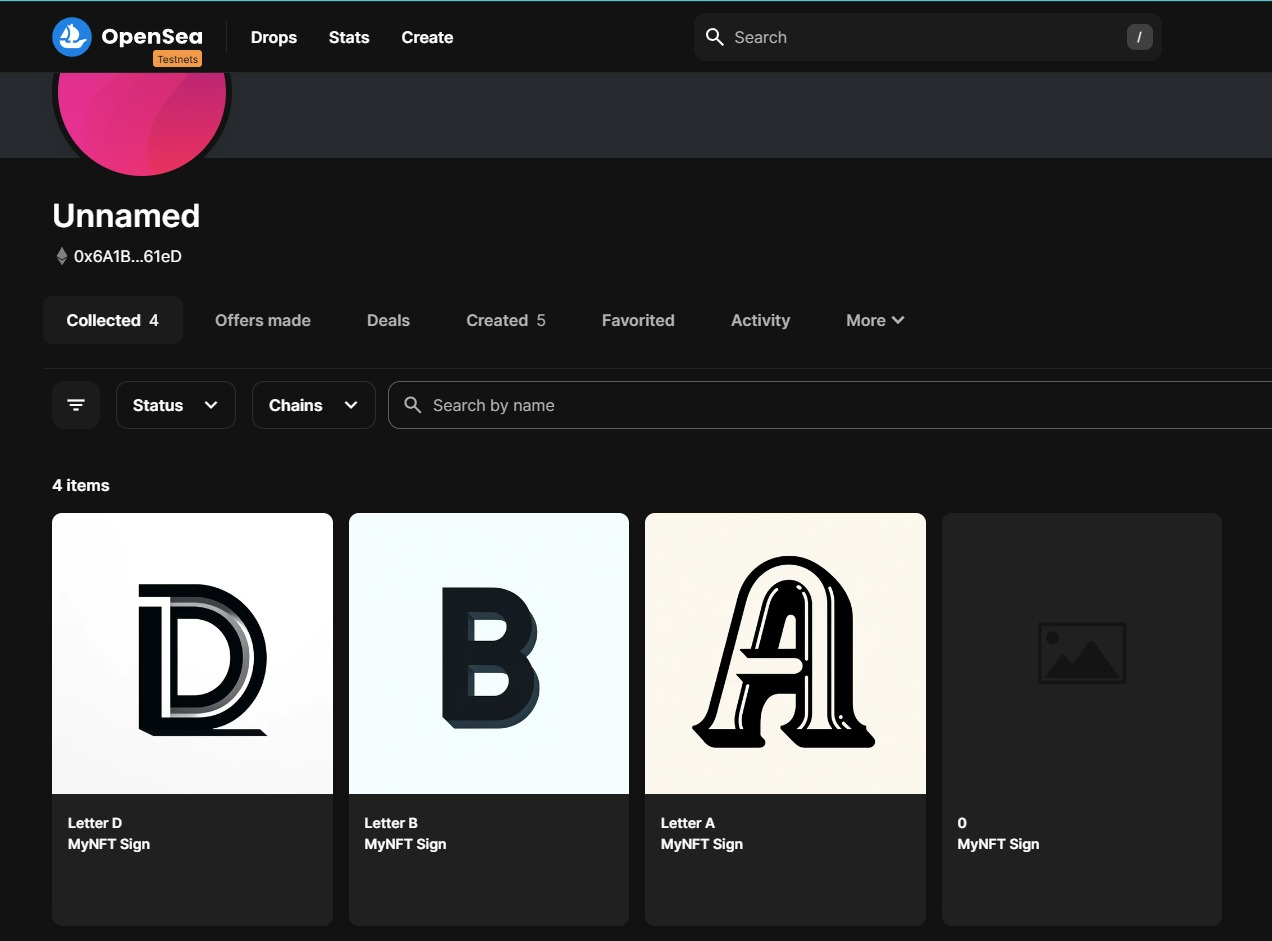
\includegraphics[scale=0.30]{gambar/nft_pada_opensea.jpeg}
    % Keterangan gambar yang diinputkan
    \caption{NFT pada OpenSea}
    % Label referensi dari gambar yang diinputkan
    \label{fig:nft_opensea}
    \end{figure}

    \item setelah NFT sudah terbuat, maka tahap berikutnya adalah melakukan \emph{lock} pada NFT yang akan dikirimkan ke \emph{user} B pada \emph{network} B'. Fungsi dari \emph{lock} ini untuk menjamin bahwa data token tidak diubah selama proses \emph{transfer}, menjaga kepercayaan dan keautentikan data NFT. Kemudian juga berguna untuk memberi sinyal kepada semua pihak terkait (pengguna, \emph{smart contract} di jaringan lain) bahwa token tersebut sedang dalam proses \emph{transfer}, dan operasi pada token harus ditangguhkan hingga proses selesai.

    \begin{figure} [H] \centering
    % Nama dari file gambar yang diinputkan
    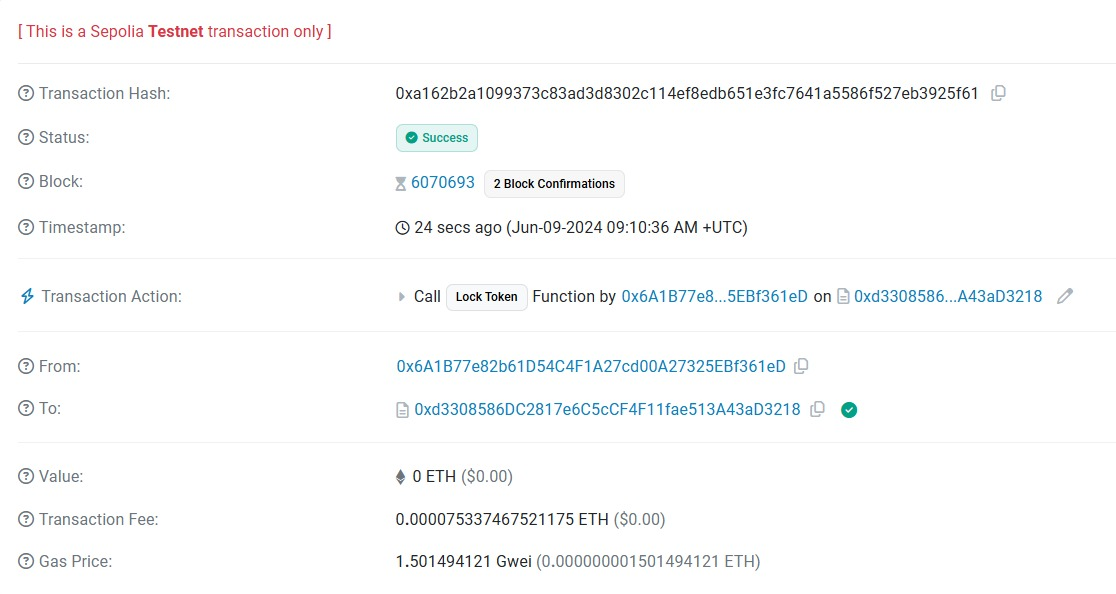
\includegraphics[scale=0.32]{gambar/lock_token.jpeg}
    % Keterangan gambar yang diinputkan
    \caption{Detail fungsi \emph{Lock Token} pada Etherscan}
    % Label referensi dari gambar yang diinputkan
    \label{fig:locktoken}
    \end{figure}

    \item selesai melakukan proses \emph{lock token}, lalu fungsi \emph{bridge transfer} dapat dilaksanakan. Fungsi ini memfasilitasi transfer aman NFT antar \emph{blockchain} dengan memastikan bahwa NFT tersebut terkunci selama proses transfer dan memberikan visibilitas transparan tentang kejadian transfer melalui \emph{event} yang dicatat. Ini adalah komponen kunci dalam membangun aplikasi \emph{interoperable} yang memungkinkan aset \emph{digital} bergerak lintas ekosistem \emph{blockchain}.

    \begin{figure} [H] \centering
    % Nama dari file gambar yang diinputkan
    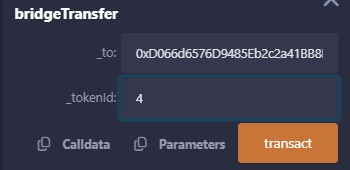
\includegraphics[scale=0.75]{gambar/bridge_transfer.jpeg}
    % Keterangan gambar yang diinputkan
    \caption{Parameter \emph{bridge transfer}}
    % Label referensi dari gambar yang diinputkan
    \label{fig:bridge_tranfer}
    \end{figure}

    \item pada gambar \ref{fig:bridge_tranfer} terdapat 2 parameter yaitu \texttt{"\emph{\_to}"}" yang digunakan untuk menerima parameter \emph{address} dari \emph{user} B dan juga parameter \texttt{"\emph{\_tokenId}"} untuk menerima argumen dari token NFT. Setelah dilakukan \emph{transact} maka akan dilanjutkan ke pembayaran pada Metamask Wallet.

    \begin{figure} [H] \centering
    % Nama dari file gambar yang diinputkan
    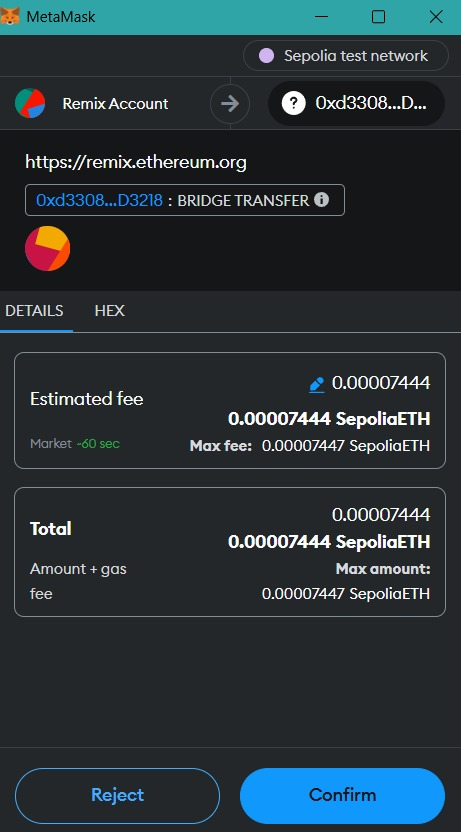
\includegraphics[scale=0.32]{gambar/verifikasi_metamask_wallet.jpeg}
    % Keterangan gambar yang diinputkan
    \caption{Pembayaran pada Metamask Wallet}
    % Label referensi dari gambar yang diinputkan
    \label{fig:metamask_pembayaran}
    \end{figure}

    \item setelah transaksi berhasil, \emph{record} dari transaksi tersimpan pada \emph{blockchain} yang dapat dilihat pada etherscan seperti pada gambar di bawah ini.

    \begin{figure} [H] \centering
    % Nama dari file gambar yang diinputkan
    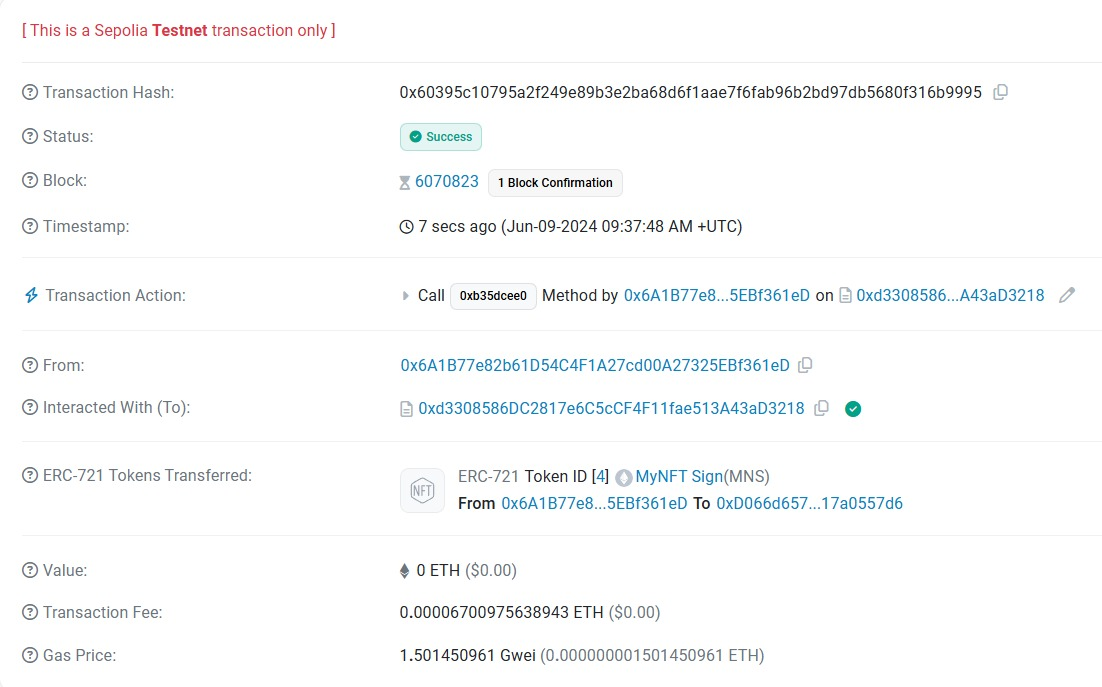
\includegraphics[scale=0.35]{gambar/detail_pada_etherscan.jpeg}
    % Keterangan gambar yang diinputkan
    \caption{Detail pada Etherscan}
    % Label referensi dari gambar yang diinputkan
    \label{fig:detail_etherscan}
    \end{figure}

    \item pada etherscan juga terdapat detail pada NFT yang dapat dicek kepemilikannya. Jika dilihat dari gambar \ref{fig:detail_nft_etherscan} \emph{owner} dari NFT \#4 adalah \emph{address} dari \emph{user} A yang berada pada \emph{network Sepolia Ethereum Testnet}, lalu pada gambar di bawah ini setelah berhasil melakukan \emph{bridge transfer} kepemilikannya berganti kepada \emph{user} B yang berada pada \emph{network BNB Chain Testnet}.

    \begin{figure} [H] \centering
    % Nama dari file gambar yang diinputkan
    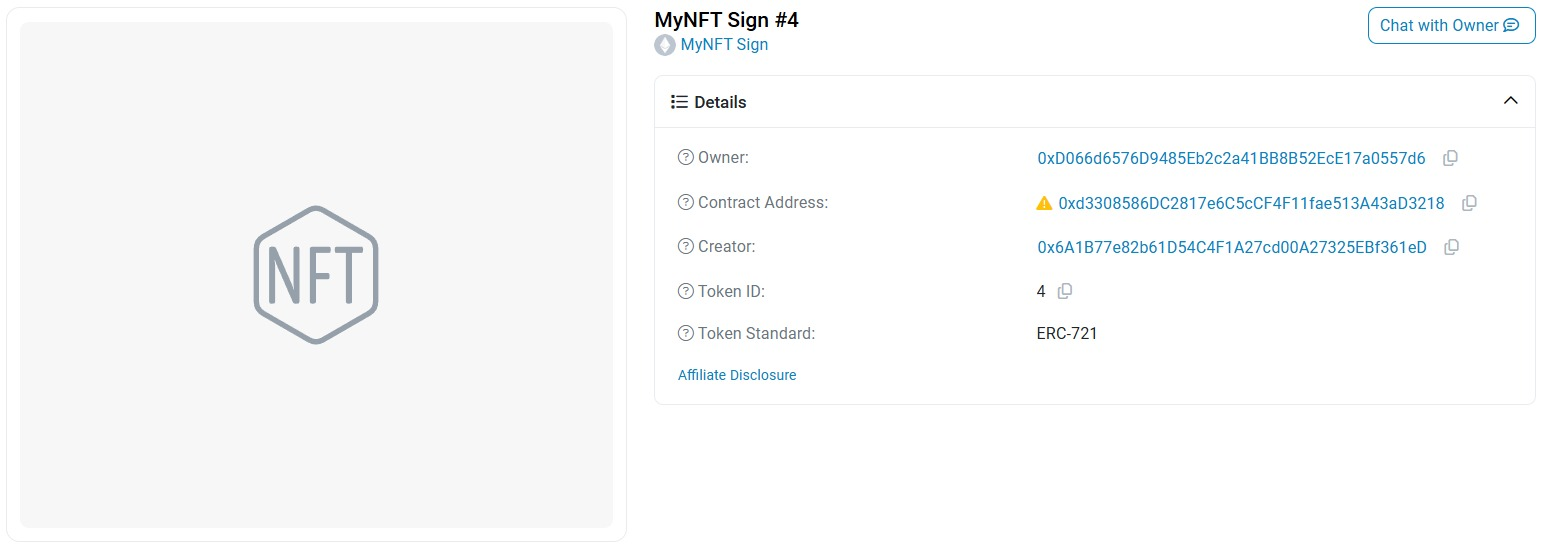
\includegraphics[scale=0.3]{gambar/nft_detail_etherscan2.jpeg}
    % Keterangan gambar yang diinputkan
    \caption{Detail NFT pada Etherscan setelah \emph{bridge transfer}}
    % Label referensi dari gambar yang diinputkan
    \label{fig:nft_bridge_transfer}
    \end{figure}

    \item pada \emph{platform} OpenSea juga dapat dilihat pada akun milik \emph{adrress} \emph{user} B maka juga terdapat NFT yang telah terkirim ke alamatnya.

    \begin{figure} [H] \centering
    % Nama dari file gambar yang diinputkan
    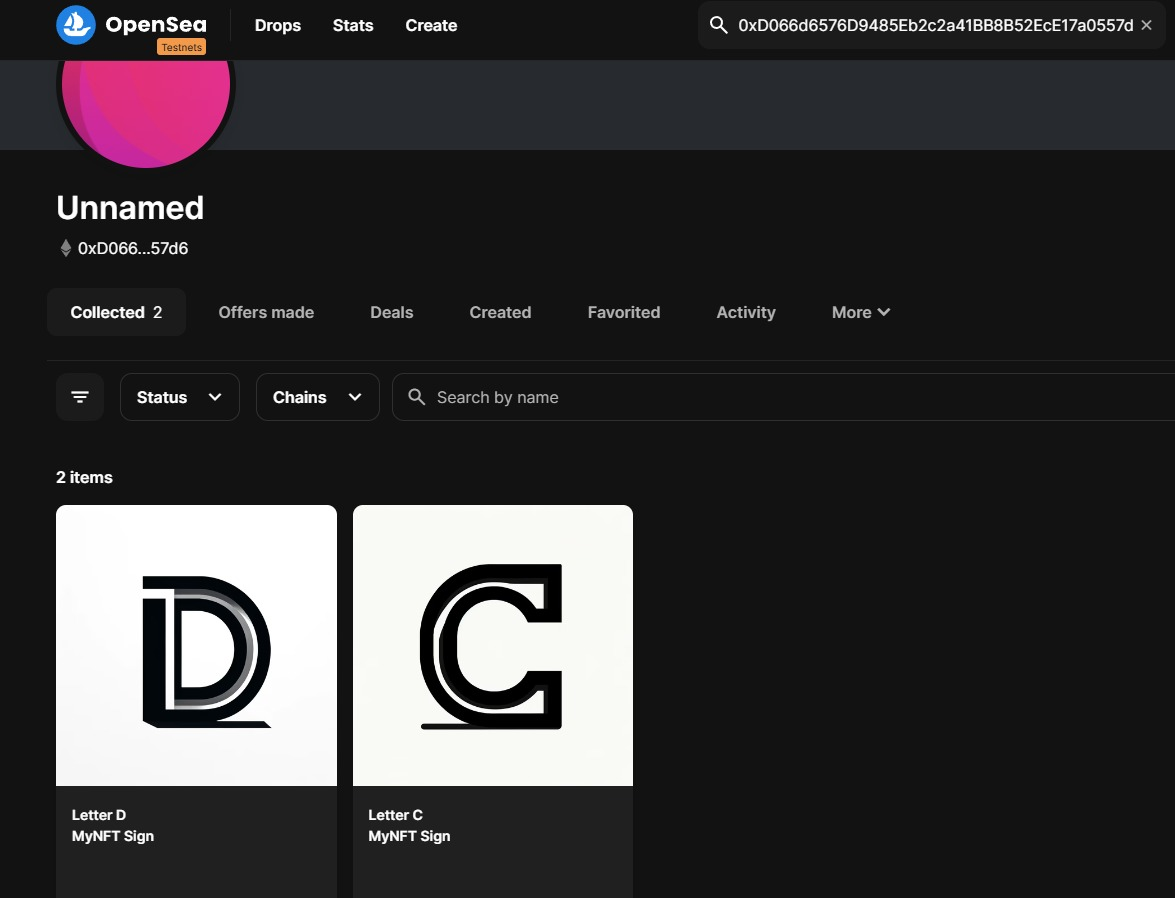
\includegraphics[scale=0.27]{gambar/nft_pada_opensea_2.jpeg}
    % Keterangan gambar yang diinputkan
    \caption{NFT pada OpenSea \emph{address} B}
    % Label referensi dari gambar yang diinputkan
    \label{fig:opensea2}
    \end{figure}
    
\end{itemize}

\subsection{Pengujian Integrasi \emph{Smart Contract} Dengan Web3.0}
Ekspektasi pengujian dari integrasi sistem \emph{smart contract} dengan web3.0 antara lain adalah sebagai berikut:
\begin{itemize}
    \item \emph{User} dapat melakukan integrasi akun Metamask Wallet dengan aplikasi web3.0

    \item \emph{User} dapat melakukan \emph{create listing} NFT untuk mengunggah NFT dari pemilik ke halaman \emph{Home} dan ke halaman \emph{My Listed Items}.

    \item \emph{User} dapat melakukan minting pada NFT yang telah dibuat dan kemudian terlihat pada halaman \emph{My Purchases}.

    \item \emph{User} yang memiliki NFT tersebut dapat melakukan \emph{transfer ownership} atau pindah kepemilikan dari alamat pengguna pemilik menuju ke alamat pengguna tujuan.

    \item \emph{User} yang memiliki NFT tersebut dapat melakukan fungsi seperti tahapan dalam melakukan \emph{bridge transfer} untuk melakukan pengiriman NFT dari alamat pengguna pada \emph{network} lokal ke alamat pengguna tujuan yang berada pada \emph{network} \emph{binance smart chain} ataupun \emph{sepolia ethereum}. 
\end{itemize}

Berikut merupakan langkah-langkah dari pengujian integrasi \emph{smart contract} dengan Web3.0 yang akan dilakukan:

\begin{itemize}
    \item \emph{User} akan mengakses web dengan menggunakan link yang dimunculkan secara lokal dengan melakukan run program lalu akan memunculkan link berupa \emph{localhost} yang dapat diakses pada platform seperti Google Chrome, Mozilla Firefox, atau Microsoft Edge, dan platform pengakses website lainnya.

    \begin{figure} [H] \centering
      % Nama dari file gambar yang diinputkan
      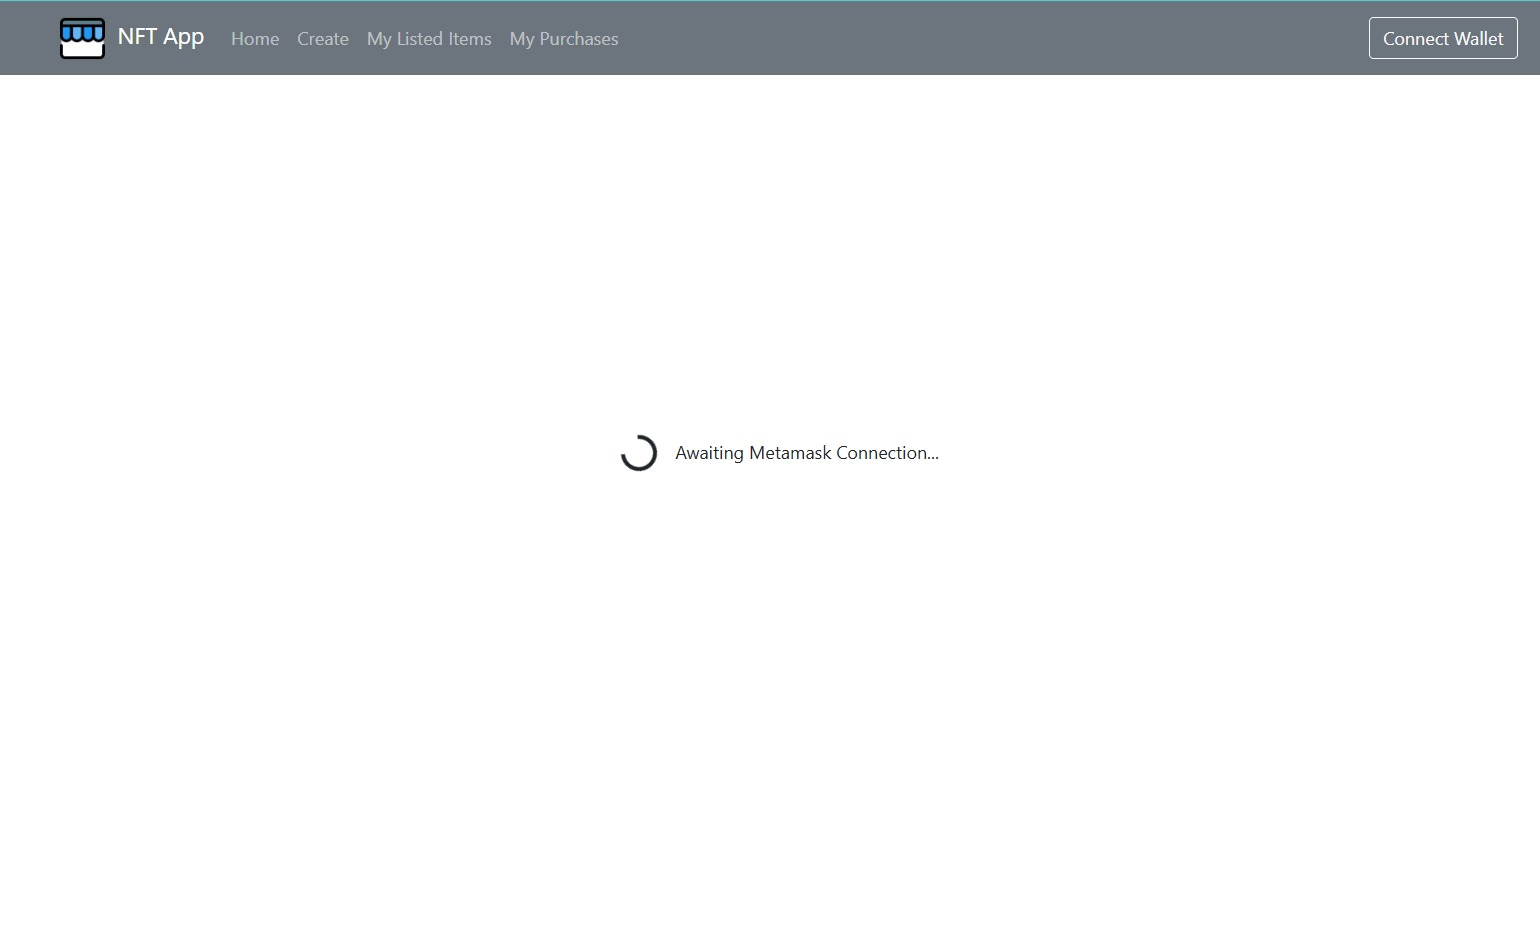
\includegraphics[scale=0.25]{gambar/login_page.jpg}
      % Keterangan gambar yang diinputkan
      \caption{Tampilan awal dari web}
      % Label referensi dari gambar yang diinputkan
      \label{fig:web_interface}
      \end{figure}

    \item Pada gambar \ref{fig:web_interface} merupakan tampilan utama dari web, sebelum dapat melakukan \emph{load} data pengguna harus melakukan koneksi dengan akun Metamask Wallet. Integrasi harus dilakukan agar pengguna dapat mengakses tampilan lanjutan pada web. Integrasi tersebut dapat dilakukan dengan menekan tombol \emph{Connect Wallet} pada \emph{navigation bar} di pojok kanan atas.
    
    \begin{figure} [H] \centering
      \centering
      \begin{subfigure}{0.45\textwidth}
          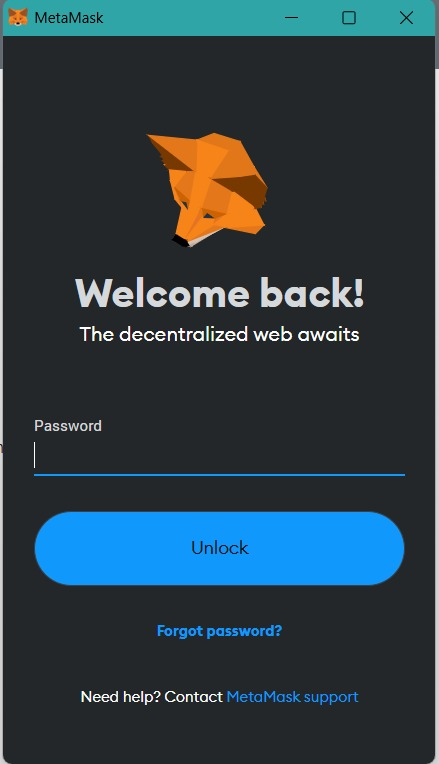
\includegraphics[scale=0.35]{gambar/integrasi_metamask.jpg}
          \caption{}
          \label{fig:intg_a}
      \end{subfigure}
      \hspace{5pt}
      \begin{subfigure}{0.45\textwidth}
        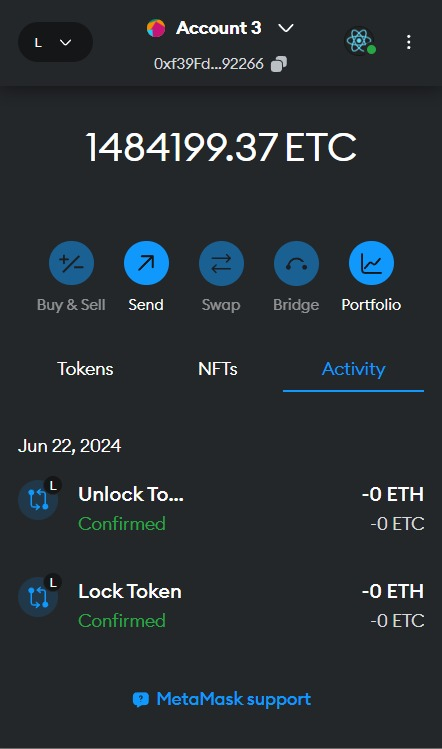
\includegraphics[scale=0.35]{gambar/metamask_konek.jpeg}
        \caption{}
        \label{fig:intg_b}
    \end{subfigure}
      \caption{Koneksi Metamask dengan Web}
      \label{fig:koneksi_web_metamask}
      \end{figure}

      \item Pada gambar \ref{fig:koneksi_web_metamask} adalah proses ketika melakukan integrasi dengan Metamask Wallet pada web. Ketika pengguna menekan tombol \emph{Connect Wallet} maka akan diarahkan kepada Metamask. Jika pengguna belum melakukan login pada Metamask maka pengguna akan disuruh login terlebih dahulu pada Metamask seperti pada gambar \ref{fig:intg_a}. Jika pengguna telah melakukan login ke akun Metamask, maka tampilannya akan seperti gambar \ref{fig:intg_b} yang di mana tampilan dari Metamask Wallet terdapat informasi \emph{address} dari akun dan juga \emph{balance} dari akun tersebut. Dikarenakan pada pengujian ini masih menggunakan \emph{localhost} maka \emph{balance} dari akun tersebut menggunakan milik Hardhat.
      
      \begin{figure} [H] \centering
        % Nama dari file gambar yang diinputkan
        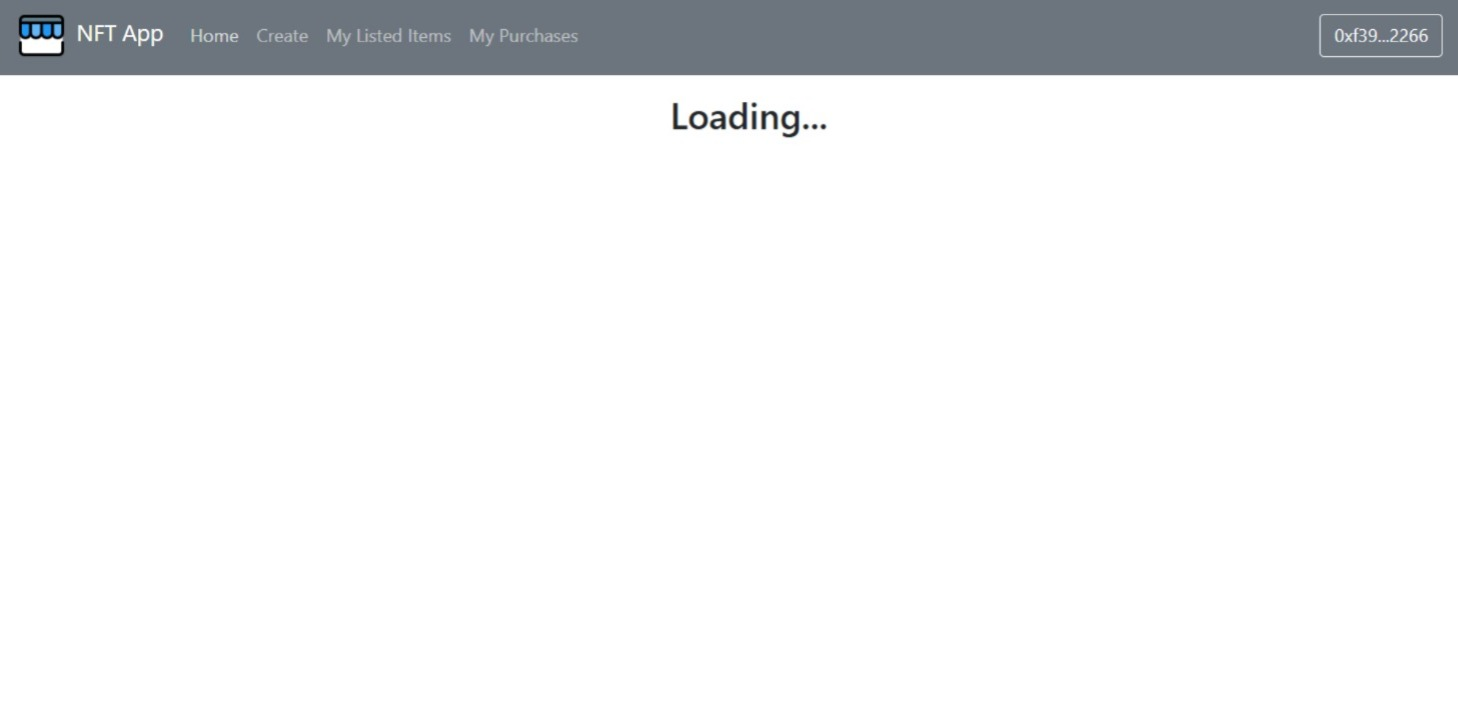
\includegraphics[scale=0.27]{gambar/home_page.jpg}
        % Keterangan gambar yang diinputkan
        \caption{Tampilan awal dari web}
        % Label referensi dari gambar yang diinputkan
        \label{fig:homepage}
        \end{figure}

        \item Pada gambar \ref{fig:homepage} adalah tampilan dari \emph{homepage} awal ketika pengguna menekan tombol \emph{home} pada \emph{navigation bar} atas. Pada web ini terdapat beberapa halaman yang dapat diakses dengan menekan tombol pada \emph{navigation bar}, seperti \emph{Home}, \emph{Create}, \emph{My Listed Items}, dan \emph{My Purchase}. Tampilan-tampilan ini dapat diakses ketika pengguna telah melakukan koneksi web dengan Metamask Wallet, hal ini dapat dilihat pada \emph{navigation bar} atas kanan terdapat \emph{address} dari akun Metamask Wallet. Pada tampilan awal ini, pengguna dapat melihat NFT yang telah diunggah untuk dapat dilakukan pembelian atau \emph{minting}. Tetapi karena belum terdapat NFT yang diunggah maka hanya akan menampilkan tulisan "\emph{Loading...}".
         
        \begin{figure} [H] \centering
          % Nama dari file gambar yang diinputkan
          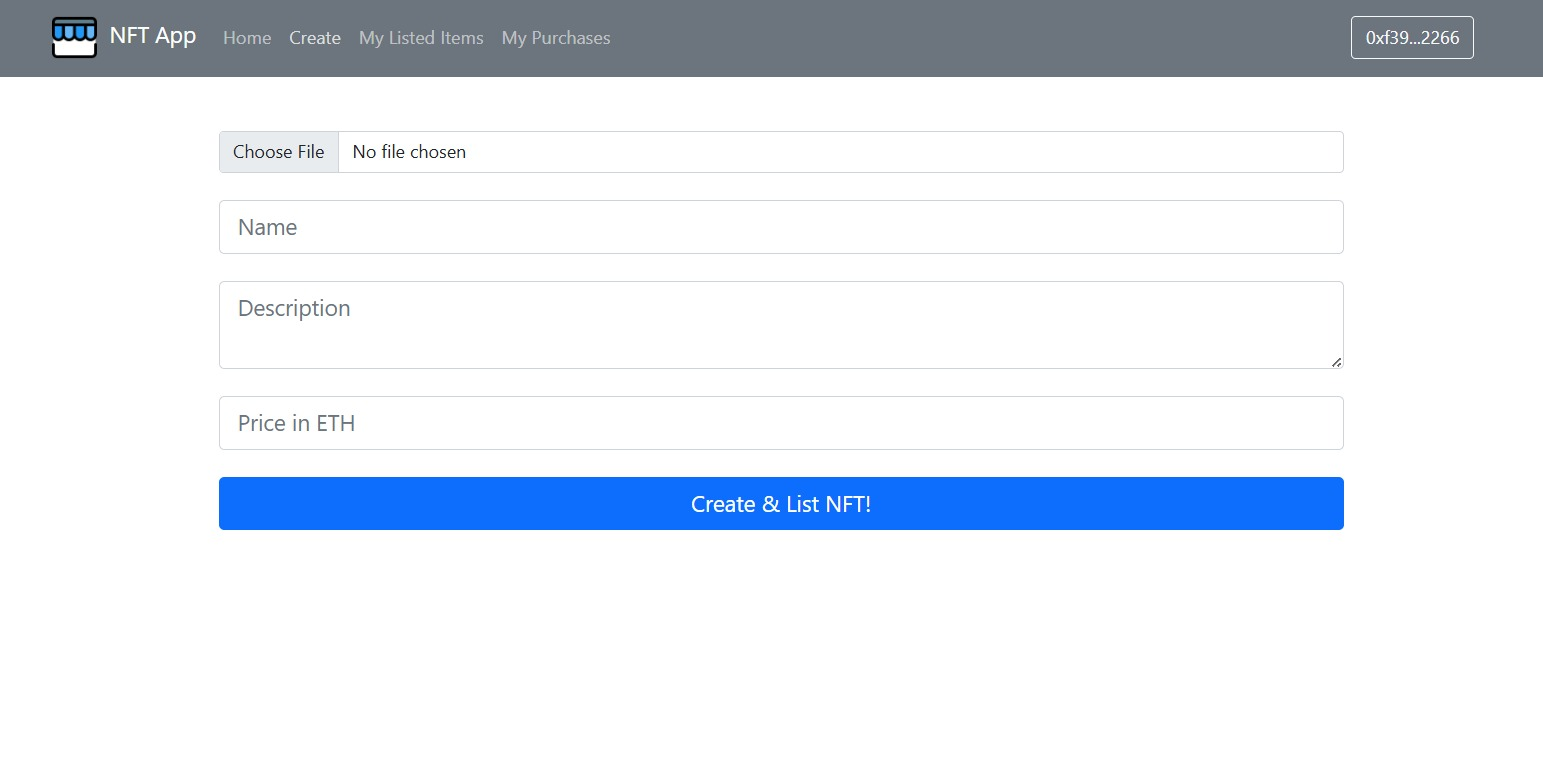
\includegraphics[scale=0.27]{gambar/create_page.jpeg}
          % Keterangan gambar yang diinputkan
          \caption{Tampilan halaman \emph{create}}
          % Label referensi dari gambar yang diinputkan
          \label{fig:createpage}
          \end{figure}

        \item Pada gambar \ref{fig:createpage} adalah tampilan dari \emph{create page}. Pada halaman ini pengguna dapat mengunggah sebuah NFT berupa gambar ke web yang kemudian jika diunggah akan muncul pada halaman \emph{home} dan juga akan muncul pada halaman \emph{my listed items}.
    
        \begin{figure} [H] \centering
          % Nama dari file gambar yang diinputkan
          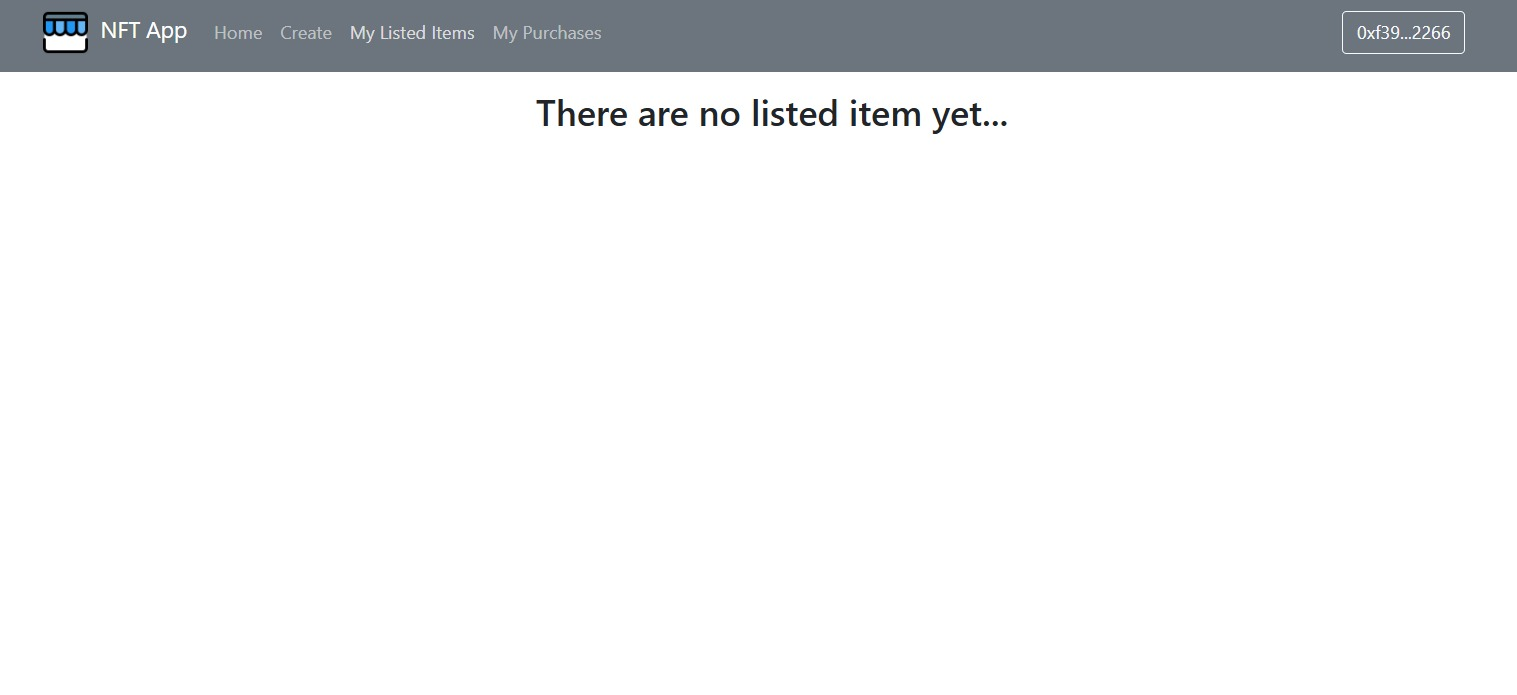
\includegraphics[scale=0.27]{gambar/listing_page.jpg}
          % Keterangan gambar yang diinputkan
          \caption{Tampilan halaman \emph{my listed items}}
          % Label referensi dari gambar yang diinputkan
          \label{fig:listingpage}
          \end{figure}
        
        \item Pada gambar \ref{fig:listingpage} adalah tampilan dari \emph{my listed items page}. Pada halaman ini pengguna dapat melihat NFT kepemilikannya yang telah diunggah pada ketika dia melakukan \emph{create}. Tetapi dikarenakan belum melakukan pengunggahan NFT, maka halaman ini hanya akan memunculkan tulisan "\emph{There are no listed item yet}".

        \begin{figure} [H] \centering
          % Nama dari file gambar yang diinputkan
          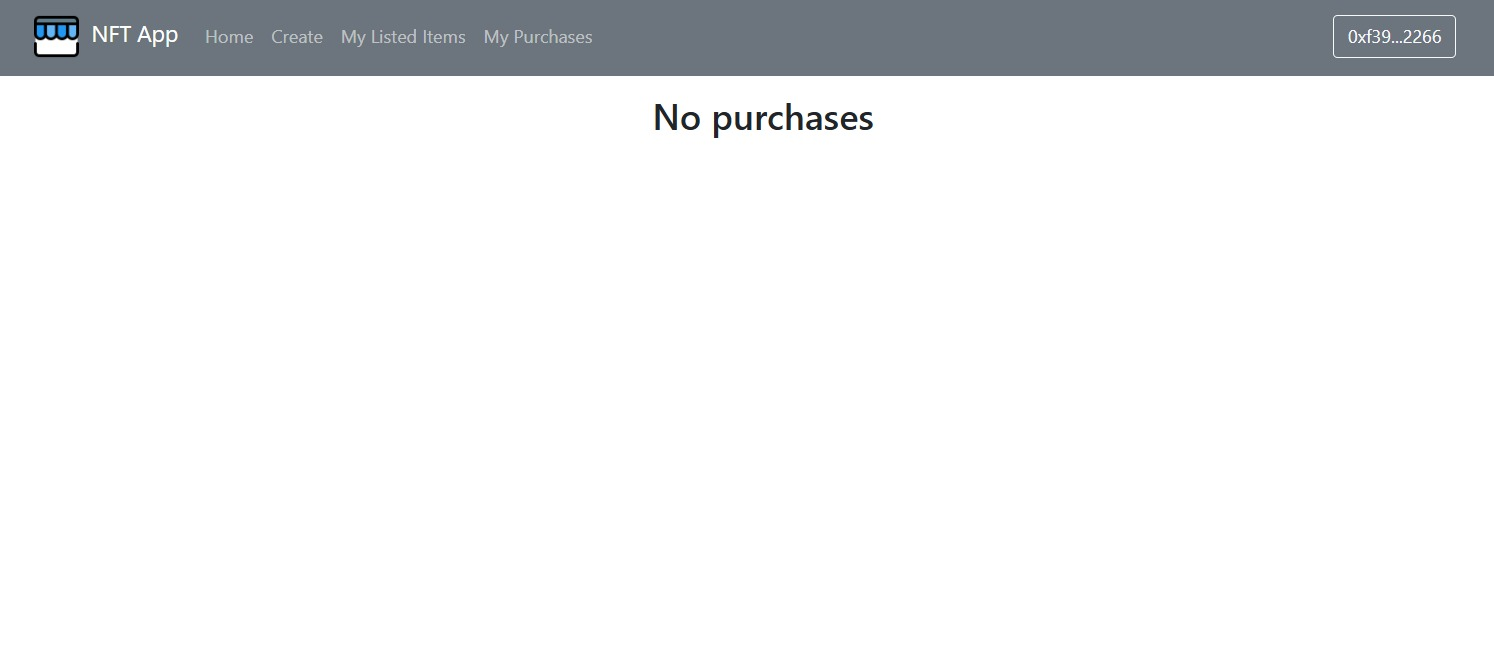
\includegraphics[scale=0.27]{gambar/purchase_page.jpg}
          % Keterangan gambar yang diinputkan
          \caption{Tampilan halaman \emph{my purchases}}
          % Label referensi dari gambar yang diinputkan
          \label{fig:purchasepage}
          \end{figure}
        
        \item Pada gambar \ref{fig:purchasepage}, terlihat tampilan dari \emph{my purchase page} yang dirancang khusus untuk memungkinkan pengguna melihat semua NFT yang telah mereka peroleh melalui pembelian di halaman utama platform. Setelah melakukan pembelian, NFT tersebut akan terdaftar di halaman ini, memberikan tampilan visual serta detail dari setiap NFT yang dimiliki. Lebih lanjut, halaman ini juga menyediakan fungsi \emph{transfer ownership}, yang memungkinkan pemilik untuk mengalihkan kepemilikan NFT kepada pengguna lain dengan \emph{address} yang berbeda. Fungsi ini sangat penting untuk mendukung fleksibilitas dan likuiditas dalam perdagangan NFT di pasar. Namun, jika pengguna belum melakukan pembelian apapun, halaman ini akan menampilkan pesan "\emph{No purchases}", yang menandakan bahwa tidak ada NFT yang dapat ditampilkan atau ditransfer.
        
        \item Kemudian, kita akan menguji fungsionalitas sistem dengan fokus pada proses pengunggahan NFT, melakukan transaksi pembelian, serta mengirim NFT ke \emph{address} lain. Dalam skenario pengujian ini, seluruh aktivitas akan dilakukan dalam jaringan yang sama, yakni \emph{localhost}. Hal ini bertujuan untuk memastikan bahwa interaksi antar fungsi dalam \emph{smart contract} berjalan dengan lancar dan tanpa adanya gangguan eksternal yang mungkin terjadi dalam jaringan publik. Pengujian di \emph{localhost} memungkinkan kita untuk mengisolasi dan mengidentifikasi masalah fungsi dalam kondisi yang terkontrol sebelum memindahkannya ke jaringan tes yang lebih besar atau ke jaringan Ethereum utama. Selama proses ini, kita akan mengamati bagaimana sistem menangani proses-proses seperti penentuan kepemilikan, transaksi pembayaran, dan transfer kepemilikan antar pengguna, yang semuanya merupakan komponen penting dari aplikasi berbasis NFT. Pengujian ini juga mencakup verifikasi keamanan dan integritas data untuk memastikan bahwa tidak ada celah yang dapat dimanfaatkan oleh pengguna jahat dalam ekosistem.
      
      \begin{figure} [H] \centering
        % Nama dari file gambar yang diinputkan
        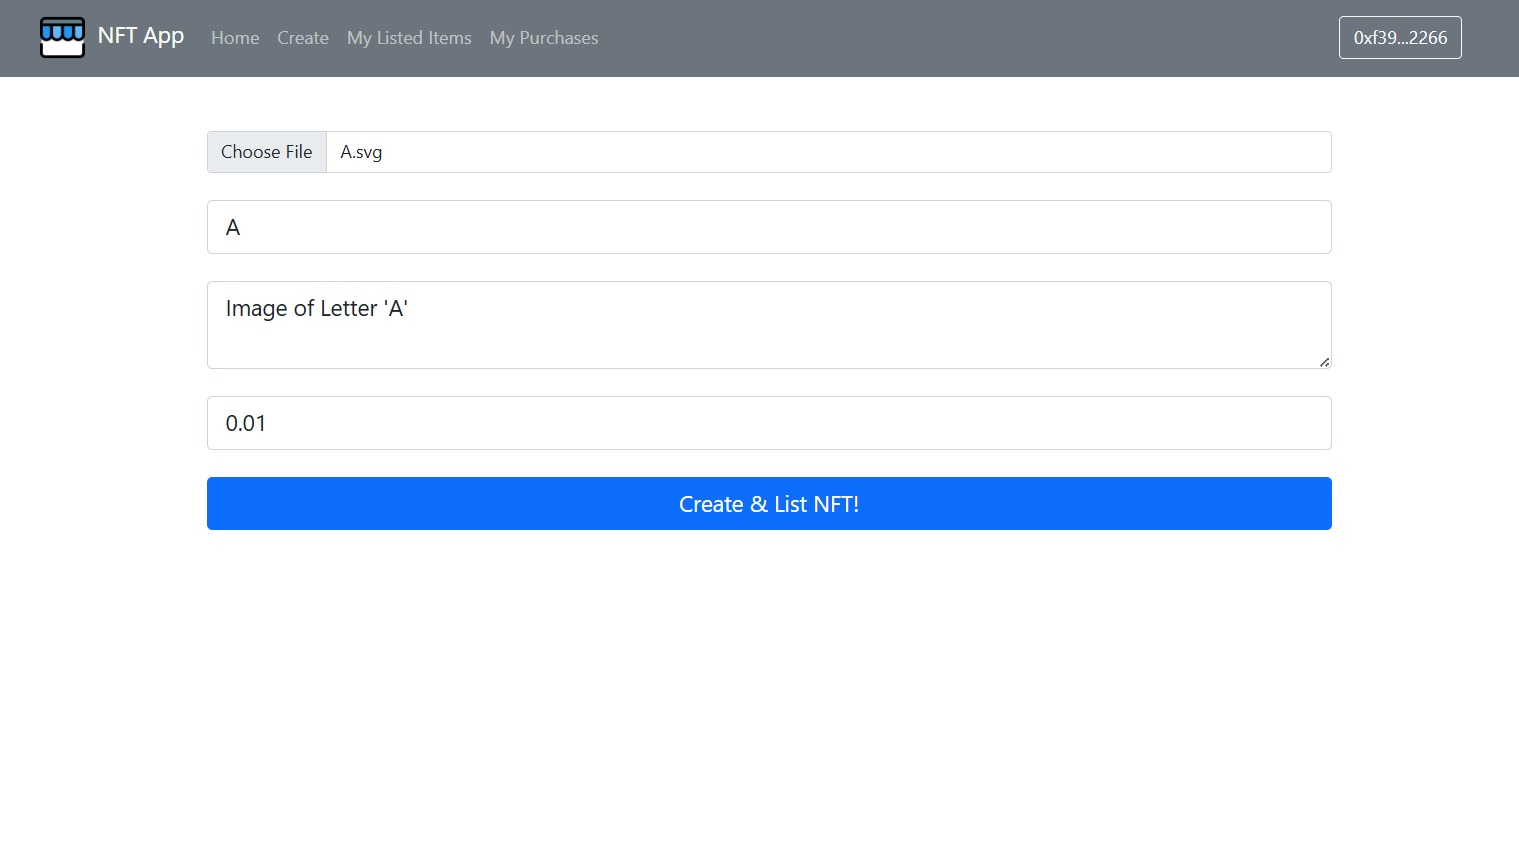
\includegraphics[scale=0.27]{gambar/create_nft.jpg}
        % Keterangan gambar yang diinputkan
        \caption{Melakukan pengunggahan NFT pada halaman \emph{create}}
        % Label referensi dari gambar yang diinputkan
        \label{fig:createnft}
        \end{figure}

      \item Pada tahap awal ini pengguna melakukan pengunggahan NFT pada halaman \emph{create}. Pengguna memasukkan detail-detail dari NFT yang ingin diunggah seperti gambar, nama, deskripsi, dan juga harga dalam mata uang \emph{ethereum}. Pada pengujian ini pengguna memasukkan NFT gambar "A" seperti pada pengujian \emph{smart contract} sebelumnya. Setelah pengguna menekan tombol "\emph{Create \& List NFT!}" maka akan muncul \emph{pop up window} dari Metamask Wallet yang digunakan untuk membayar \emph{gas} atau fee dari melakukan eksekusi kode \emph{smart contract}. 
      
       \begin{figure} [H] \centering
      \centering
      \begin{subfigure}{0.45\textwidth}
          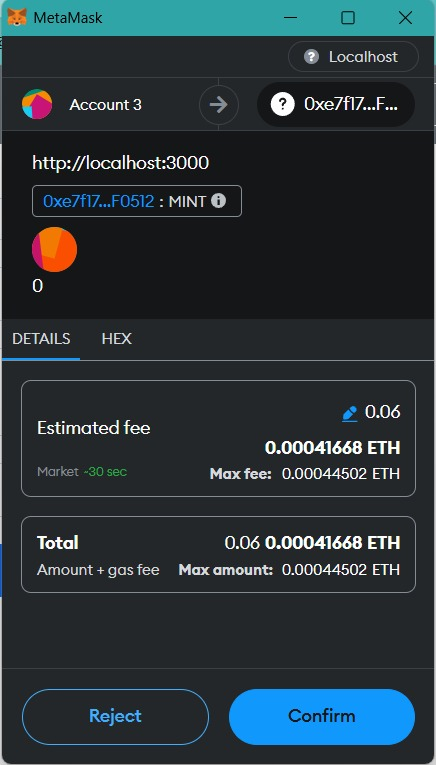
\includegraphics[scale=0.32]{gambar/confirm_create.jpg}
          \caption{}
          \label{fig:payipfs-a}
      \end{subfigure}
      \hspace{5pt}
      \begin{subfigure}{0.45\textwidth}
        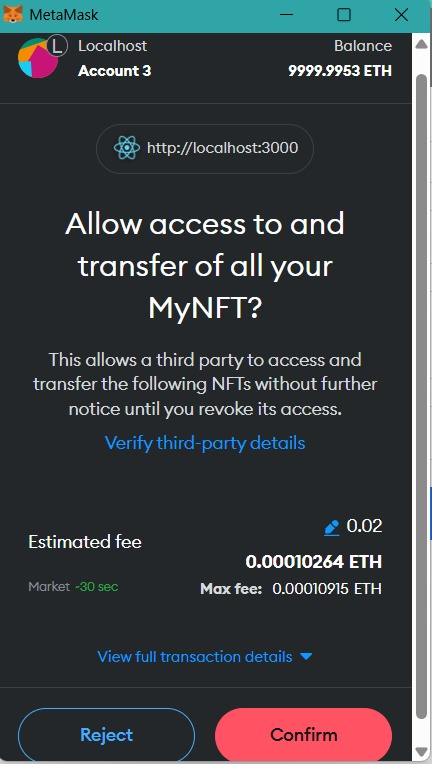
\includegraphics[scale=0.32]{gambar/confirm_upload.jpg}
        \caption{}
        \label{fig:payipfs-b}
    \end{subfigure}
      \caption{Pembayaran gas IPFS menggunakan Metamask Wallet}
      \label{fig:koneksi_web_metamask}
      \end{figure}
      
        \item Gambar \ref{fig:payipfs-a} adalah pembayaran \emph{gas} dari metamask wallet. Pembayaran \emph{gas} tersebut terjadi karena pada \emph{smart contract} terjadi proses pengunggahan gambar NFT ke platform penyedia IPFS. Pada web ini kita mengintegrasikan dengan platform bernama Pinata. Pinata sendiri merupakan platform penyedia servis IPFS. Kemudian juga terdapat konfirmasi pada gambar \ref{fig:payipfs-b}, konfirmasi ini dilakukan karena melakukan integrasi dengan platform Pinata yang kita gunakan sebagai penyedia servis IPFS. 
        
        \item Setelah berhasil melakukan konfirmasi pembayaran gas melalui MetaMask, NFT yang telah dibuat melalui halaman "Create" pada aplikasi akan diunggah ke platform Pinata. Platform Pinata ini berfungsi sebagai penyedia layanan penyimpanan dan pengelolaan file berbasis teknologi blockchain, yang menggunakan sistem InterPlanetary File System (IPFS) untuk memastikan keamanan dan ketahanan data.
        
        \begin{figure} [H] \centering
          % Nama dari file gambar yang diinputkan
          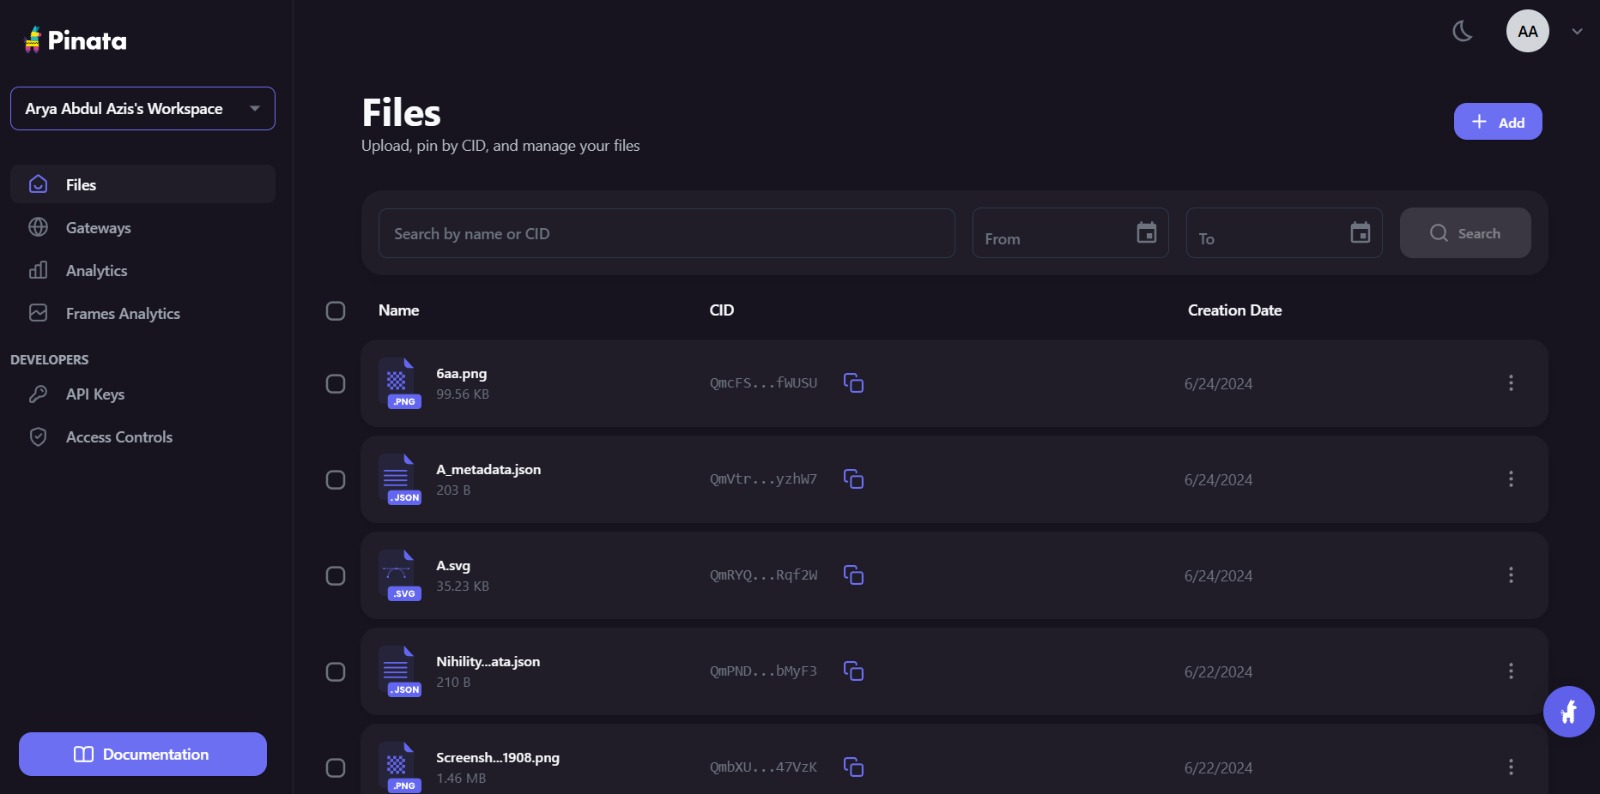
\includegraphics[scale=0.26]{gambar/pinata.jpeg}
          % Keterangan gambar yang diinputkan
          \caption{Data dari NFT ter-\emph{upload} pada platform Pinata}
          % Label referensi dari gambar yang diinputkan
          \label{fig:pinata}
          \end{figure}

        \item Dalam platform Pinata seperti pada gambar \ref{fig:pinata}, setiap file yang diunggah, termasuk gambar untuk NFT, akan diberikan Content Identifier (CID) unik yang memudahkan pelacakan dan akses tanpa perlu mengkhawatirkan perubahan isi file, karena CID ini akan berubah jika konten file berubah. Hal ini sangat penting dalam ekosistem NFT di mana keaslian dan keunikan konten harus terjamin. Di Pinata, pengguna dapat dengan mudah melihat semua file yang telah diunggah, mengatur akses, dan memantau penggunaan dan analisis lalu lintas file. Fitur ini memungkinkan pembuat konten NFT untuk tidak hanya menyimpan aset digital mereka dengan aman tetapi juga mengelola distribusi mereka dengan lebih efektif dalam pasar digital. Keseluruhan proses ini mengintegrasikan teknologi blockchain dengan aplikasi web, memastikan bahwa setiap pembelian dan transfer NFT dapat dilacak dan diverifikasi secara transparan dan aman. Pinata tidak hanya menyediakan solusi penyimpanan yang efisien dan aman tetapi juga menawarkan antarmuka yang ramah pengguna, memudahkan para pengguna, terutama para pembuat NFT, untuk mengunggah dan mengelola aset digital mereka dengan mudah. Fitur pencarian dan pengelolaan file yang intuitif memungkinkan pengguna untuk mengakses dan mengatur koleksi NFT mereka tanpa hambatan, memastikan bahwa aset digital dapat dikelola dan diakses dengan cepat sesuai kebutuhan. Lebih lanjut, Pinata mendukung integrasi dengan berbagai platform dan marketplace NFT, sehingga memperluas jangkauan dan visibilitas aset digital yang disimpan di dalamnya. Hal ini memberikan nilai tambah bagi para pembuat dan kolektor NFT dalam mendistribusikan dan memperdagangkan karya mereka di berbagai platform dengan mudah dan aman. Melalui Pinata, pembuat NFT dapat memastikan bahwa setiap aset digital tidak hanya aman tetapi juga siap untuk diintegrasikan dan digunakan dalam ekosistem blockchain yang lebih luas.
      
        \begin{figure} [H] \centering
          % Nama dari file gambar yang diinputkan
          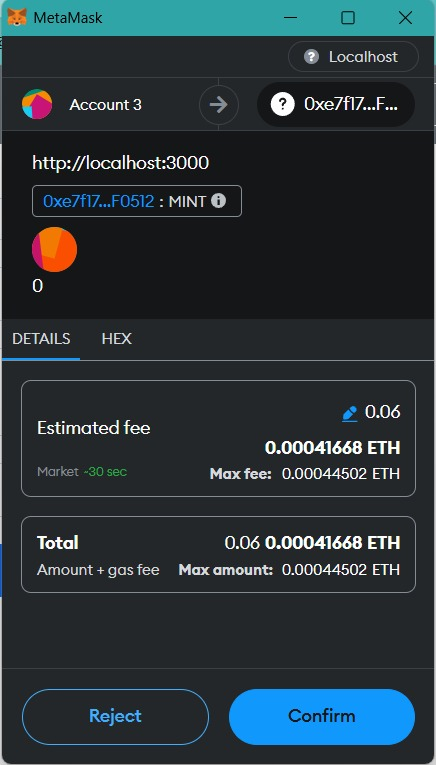
\includegraphics[scale=0.3]{gambar/confirm_create.jpg}
          % Keterangan gambar yang diinputkan
          \caption{Melakukan konfirmasi \emph{minting} NFT pada Metamask Wallet}
          % Label referensi dari gambar yang diinputkan
          \label{fig:makenft}
          \end{figure}
      
      \item 
      Pada gambar \ref{fig:makenft}, ditampilkan jendela konfirmasi MetaMask yang digunakan untuk memberikan persetujuan atas transaksi minting NFT. Dalam jendela ini, pengguna diminta untuk mengkonfirmasi atau menolak transaksi yang sedang diinisiasi dari aplikasi yang dihosting pada localhost:3000. Proses ini memastikan bahwa pengguna memahami dan menyetujui semua detail transaksi sebelum melanjutkan. Di dalam jendela konfirmasi, jumlah ETH yang akan ditransfer adalah 0, yang menandakan bahwa transaksi ini mungkin hanya melibatkan biaya gas, tanpa ada transfer dana tambahan yang terlibat. "Estimated fee" atau perkiraan biaya gas untuk transaksi ini ditampilkan, dengan jumlah minimal yang ditetapkan serta maksimum yang mungkin diperlukan, memberikan transparansi tentang biaya yang dapat dikeluarkan untuk memproses transaksi ini. Selain itu, MetaMask juga menyediakan informasi mengenai durasi estimasi untuk penyelesaian transaksi di pasar yang ditandai dengan "+30 sec", yang berarti transaksi diharapkan terjadi dalam waktu sekitar 30 detik.

      \item Setelah pengguna menyelesaikan proses minting NFT dan melakukan konfirmasi melalui MetaMask seperti yang dijelaskan sebelumnya, NFT yang baru dibuat akan muncul pada halaman "My Listed Items" dalam aplikasi. Halaman ini berfungsi sebagai galeri pribadi pengguna dimana semua NFT yang telah mereka buat dan daftarkan untuk dijual ditampilkan. Dalam contoh yang ditampilkan pada gambar, NFT dengan desain huruf "A" yang telah berhasil di-list tampak dengan harga yang tertera di bawah gambar yaitu 0.0101 ETH. Hal ini menandakan bahwa NFT ini siap untuk dibeli oleh pengguna lain. Setiap NFT yang terdaftar di halaman ini akan menampilkan gambar yang berkaitan dengan NFT tersebut, yang merupakan hasil unggahan pengguna ke IPFS, dan metadata lainnya seperti nama dan deskripsi juga akan ditampilkan jika pengguna telah menyertakannya saat proses minting.
      
      \begin{figure} [H] \centering
        % Nama dari file gambar yang diinputkan
        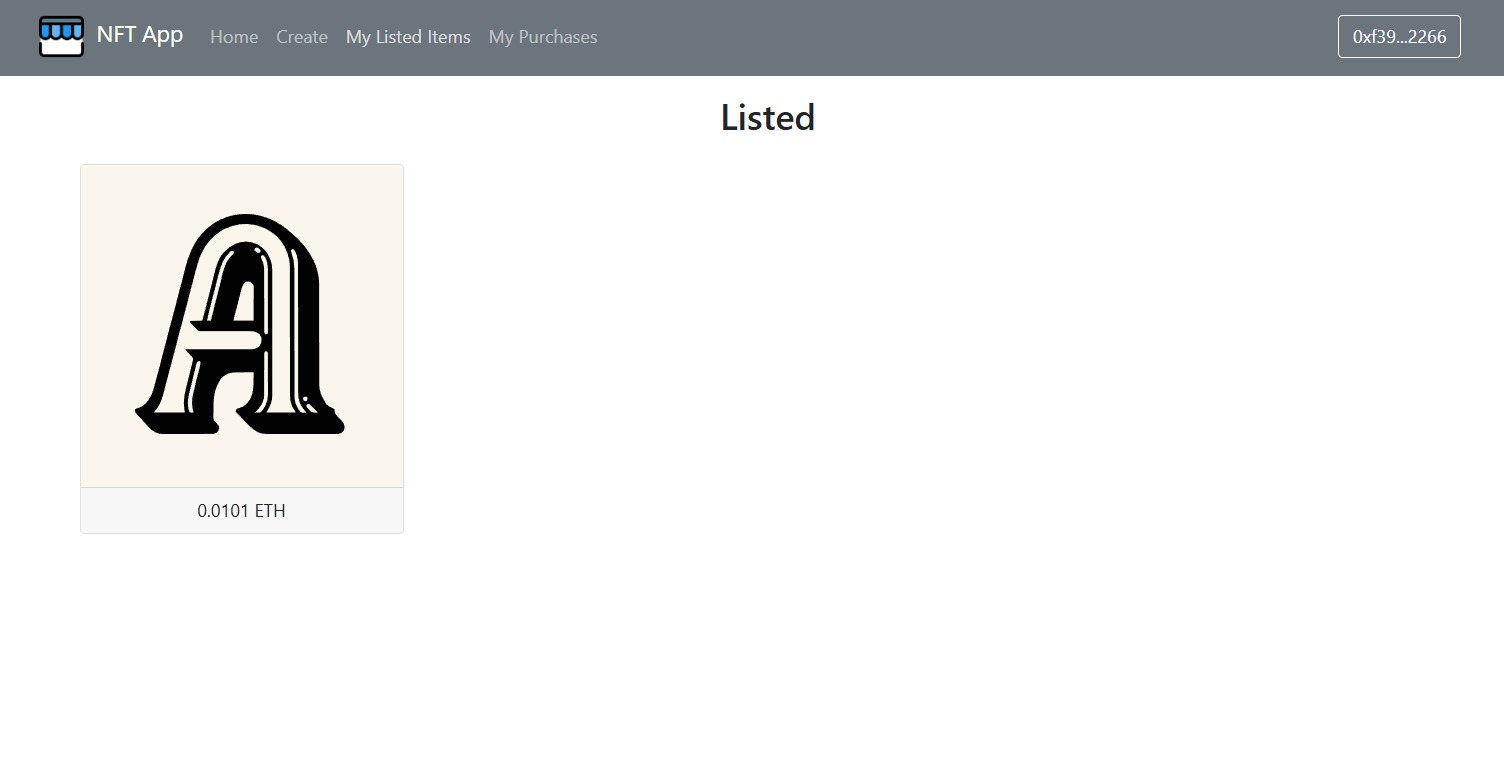
\includegraphics[scale=0.26]{gambar/listed_nft.jpg}
        % Keterangan gambar yang diinputkan
        \caption{NFT yang telah di-\emph{minting} terlihat pada halaman \emph{My listed items}}
        % Label referensi dari gambar yang diinputkan
        \label{fig:listeditem}
        \end{figure}

      \item Setelah menyelesaikan proses pengunggahan dan minting NFT, NFT yang baru dibuat juga dapat dilihat di halaman utama (\emph{home page}) web aplikasi NFT. Gambar yang disajikan menunjukkan NFT berupa gambar huruf "A", yang ditampilkan dengan label dan harga penjualan. Di halaman utama ini, NFT tidak hanya dipamerkan tetapi juga siap untuk dibeli oleh pengguna lain. Dalam tampilan ini, setiap NFT yang di-list akan dilengkapi dengan tombol "\emph{Buy}" yang memungkinkan pengguna langsung membeli NFT tersebut. Tombol ini memfasilitasi pembelian langsung tanpa perlu navigasi ke halaman lain, memberikan kemudahan bagi pembeli untuk segera mengakuisisi aset digital yang diinginkan. 
      

      \begin{figure} [H] \centering
        % Nama dari file gambar yang diinputkan
        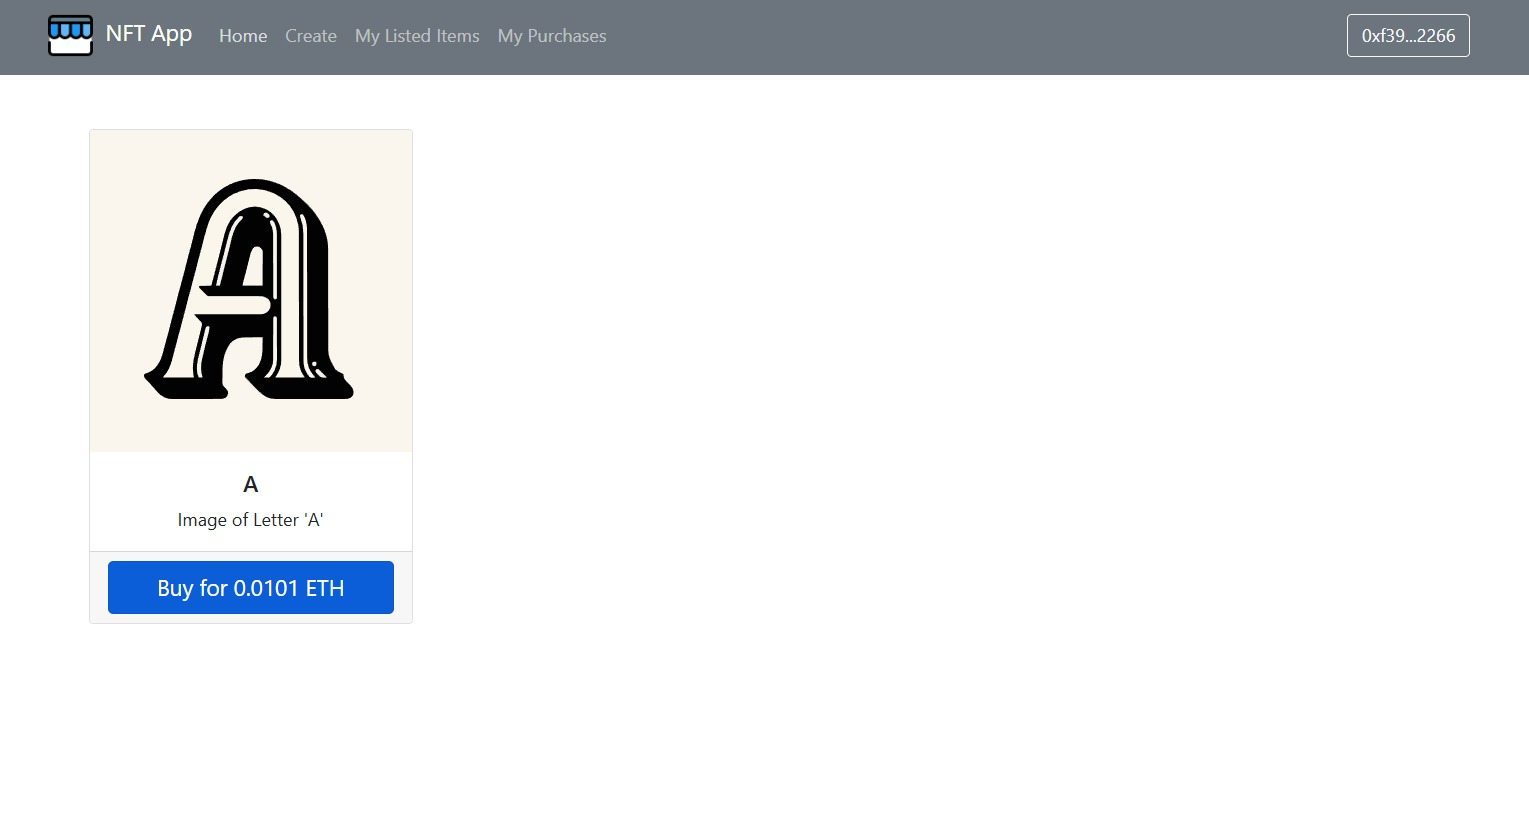
\includegraphics[scale=0.26]{gambar/nft_listed_home.jpg}
        % Keterangan gambar yang diinputkan
        \caption{NFT yang telah di-\emph{minting} terlihat pada halaman \emph{home}}
        % Label referensi dari gambar yang diinputkan
        \label{fig:listhome}
        \end{figure}


      \item Pada gambar \ref{fig:listhome} ketika tombol tersebut diklik, transaksi akan diproses melalui MetaMask atau wallet digital lainnya yang telah disinkronkan dengan aplikasi. Halaman ini dirancang untuk memberikan pengalaman pengguna yang intuitif dan efisien, di mana pembeli dapat dengan cepat mengakses NFT yang mereka inginkan dan melihat informasi penting seperti nama, deskripsi, dan harga NFT. Ini tidak hanya memperkuat transparansi dan aksesibilitas dalam pasar NFT tetapi juga mendorong interaksi langsung dan spontan antara pembeli dan aset digital.

\end{itemize}